% !TeX program = xelatex
% Adapted from Mahdi Hasanzadeh's September 2025 NCAT template (CC BY 4.0).
% Proposal author: Brandon L. Byrd. Formatting reference: NCAT Word template, 02-2026.
\documentclass[12pt,letterpaper,oneside]{report}
% NCAT February 2026 Word template governs structure and page numbering.
\usepackage[margin=1in,headheight=15pt,headsep=0.25in]{geometry}
\usepackage{fontspec}
\setmainfont{Times New Roman}
\setsansfont{Times New Roman}
\setmonofont{Times New Roman}
\usepackage{amsmath}
\usepackage{unicode-math}
\setmathfont{TeX Gyre Termes Math}
\usepackage{setspace}
\doublespacing
\usepackage{ragged2e,indentfirst}
\setlength{\JustifyingParindent}{0.5in}
\AtBeginDocument{\justifying}
\setlength{\parindent}{0.5in}
\setlength{\parskip}{0pt}
\usepackage{graphicx}
\graphicspath{{Fig/}}
\usepackage{caption}
\captionsetup{font={normalsize,doublespacing},labelfont=bf,labelsep=colon,justification=centering}
\usepackage{booktabs,array,longtable,tabularx}
\usepackage{titlesec}
\titleformat{\chapter}[block]{\normalfont\normalsize\bfseries\centering}{CHAPTER \thechapter:}{0.5em}{}
\titleformat{name=\chapter,numberless}[block]{\normalfont\normalsize\bfseries\centering}{}{0pt}{}
\titlespacing*{\chapter}{0pt}{0pt}{12pt}
\titleformat{\section}{\normalfont\normalsize\bfseries}{\thesection}{0.5em}{}
\titlespacing*{\section}{0pt}{12pt}{0pt}
\setcounter{secnumdepth}{3}
\setcounter{tocdepth}{3}
\usepackage{chngcntr}
\counterwithout{figure}{chapter}
\counterwithout{table}{chapter}
\usepackage{placeins}
\usepackage{fancyhdr}
\pagestyle{fancy}
\fancyhf{}
\fancyhead[R]{\thepage}
\renewcommand{\headrulewidth}{0pt}
\fancypagestyle{plain}{\fancyhf{}\fancyhead[R]{\thepage}\renewcommand{\headrulewidth}{0pt}}
\usepackage[nottoc,notbib]{tocbibind}
\usepackage[titles]{tocloft}
\renewcommand{\contentsname}{Table of Contents}
\renewcommand{\cftchappresnum}{CHAPTER\space}
\renewcommand{\cftchapaftersnum}{:}
\setlength{\cftchapnumwidth}{7em}
\renewcommand{\cftchapfont}{\normalfont}
\renewcommand{\cftchappagefont}{\normalfont}
\renewcommand{\cftchapleader}{\cftdotfill{\cftdotsep}}
\renewcommand{\cftfigpresnum}{Figure\space}
\renewcommand{\cftfigaftersnum}{:}
\setlength{\cftfignumwidth}{4.7em}
\renewcommand{\cfttabpresnum}{Table\space}
\renewcommand{\cfttabaftersnum}{:}
\setlength{\cfttabnumwidth}{4.7em}
\usepackage[backend=biber,style=ieee,sorting=none,maxnames=6]{biblatex}
\addbibresource{bib/references.bib}
\AtBeginBibliography{\singlespacing\justifying\interlinepenalty=10000}
\setlength{\bibitemsep}{\baselineskip}
\usepackage[hidelinks]{hyperref}
\urlstyle{same}
\setlength{\emergencystretch}{2em}
\setcounter{topnumber}{3}
\renewcommand{\topfraction}{0.9}
\renewcommand{\textfraction}{0.07}
\renewcommand{\floatpagefraction}{0.7}

\newcommand{\ThesisTitle}{Long-Tail Compositional Road-Event Detection:}
\newcommand{\ThesisSubtitle}{A Decoupled Hybrid with Learned and Semantic Composition on ROAD-Waymo}
\newcommand{\AuthorName}{Brandon L. Byrd}
\newcommand{\DegreeType}{Master of Science}
\newcommand{\ProgramName}{Computer Science}
\newcommand{\MajorProfessor}{Dr. Hamidreza Moradi}
\newcommand{\University}{North Carolina Agricultural and Technical State University}
\newcommand{\LocationCity}{Greensboro, North Carolina}
\newcommand{\GradYear}{2026}
\hypersetup{pdftitle={\ThesisTitle\space\ThesisSubtitle},pdfauthor={\AuthorName}}
\begin{document}
\pagenumbering{roman}
\hypersetup{pageanchor=false}
\thispagestyle{empty}
\begin{center}
\ThesisTitle\space\ThesisSubtitle\par
\vspace{0.20in}
\AuthorName\par
\vspace{0.35in}
\University\par
\vspace{0.35in}
A thesis submitted to the graduate faculty\par
in partial fulfillment of the requirements for the degree of\par
\DegreeType\par
Program: \ProgramName\par
Major Professor: \MajorProfessor\par
\vspace{0.35in}
\LocationCity\par
\GradYear
\end{center}

\clearpage
\hypersetup{pageanchor=true}
\setcounter{page}{2}
% Single faculty column; combined roles are explicitly allowed by the template.
\NCATfrontline{96.5}{c}{This is to certify that the master's thesis of}
\NCATfrontline{137.9}{c}{\AuthorName}
\NCATfrontline{179.3}{c}{has met the thesis requirements of}
\NCATfrontline{193.1}{c}{\University}
\NCATfrontline{234.5}{c}{\LocationCity}
\NCATfrontline{248.3}{c}{\GradYear}
\NCATfrontline{289.7}{c}{Approved by:}
\NCATfrontline{317.3}{l}{Dr. Hamidreza Moradi}
\NCATfrontline{331.1}{l}{Major Professor}
\NCATfrontline{358.7}{l}{Dr. Xiaohong Yuan}
\NCATfrontline{372.5}{l}{Committee Member}
\NCATfrontline{400.1}{l}{Dr. Kaushik Roy}
\NCATfrontline{413.9}{l}{Committee Member \& Department Chair}
\NCATfrontline{441.5}{l}{Dr. Clay S. Gloster, Jr.}
\NCATfrontline{455.3}{l}{Dean, The Graduate College}
\null

\clearpage
% The supplied template places this block at the bottom, aligned right.
\NCATfrontline{634.7}{r}{\textcopyright\ Copyright by}
\NCATfrontline{662.3}{r}{\AuthorName}
\NCATfrontline{689.9}{r}{\GradYear}
\null

\clearpage
\chapter*{Abstract}

Road-event detection requires identifying agents, their actions, their scene locations, and the compositions formed by these labels. In ROAD-Waymo, unequal training support makes rare compositions difficult to recognize even when overall detection improves. This thesis investigates how decoupled localization, learned composition, and language-informed contextual representations affect recognition of these events.

A YOLOv8x detector supplies candidate boxes and agent identities, while separately trained event heads use frozen video features. The study progresses from overlap-based score transfer and direct region classification to crop-based semantic classification, scene and language attention, and complementary expert blending. The final Contextual Semantic Expert Blend combines a dynamic-class-balancing classification expert with a second expert trained using an additional visual--phrase contrastive objective. A held-out training partition selects one fixed probability-blending weight per seed. Larger paired video and text encoders supply the final system's frozen representations.

Evaluation uses frame-level mean average precision at intersection-over-union 0.5 on 36,717 shared ROAD-Waymo validation frames. The final three-seed mean reaches 15.75\% triplet mAP and 9.00\% mean AP over the 47 triplet classes below the geometric mean training frequency, compared with 7.54\% and 4.14\% for the replicated joint baseline. Relative to the original-encoder DCB blend, triplet mAP increases by 2.32 percentage points; approximately 65\% of that increase comes from tail classes, while common-class performance also improves. Controlled comparisons show that the benefit depends on how language, context, and the loss are combined: phrase-score fusion alone gives small changes, and DCB with the original encoders improves overall performance while reducing tail performance. These results support complementary contextual representations and expert predictions under the studied protocol, with limitations from validation reuse, fixed-vocabulary evaluation, and system-level changes in the scaling comparison.

\clearpage
\chapter*{Biographical Sketch}

Brandon L. Byrd holds an Associate of Applied Science in Aircraft Maintenance Technology from the Community College of the Air Force and a Bachelor of Science in Computer Science from North Carolina Agricultural and Technical State University. He is pursuing a Master of Science in Computer Science at North Carolina Agricultural and Technical State University under the supervision of Dr. Hamidreza Moradi. His research focuses on autonomous-driving perception and compositional road-event detection. His thesis investigates a decoupled detection and classification pipeline and the use of semantic structure for rare event categories.

\clearpage
\chapter*{Dedication}

In memory of Professor Leflore, whose Python 163 course challenged me deeply and helped shape my growth as a computer scientist.

\clearpage
\chapter*{Acknowledgments}

I thank my advisor and committee chair, Dr. Hamidreza Moradi, for his guidance in developing this research. I am grateful to Dr. Xiaohong Yuan, with whom I began my research journey. I also thank Dr. Kaushik Roy for the opportunity to conduct undergraduate research with him, for encouraging me to pursue graduate school, and for the advice that helped me succeed in my courses. I appreciate his continued support as a member of my thesis committee.

I acknowledge the support of the GEM Fellowship and the opportunity to collaborate with Dr. Sun Yi in the Department of Mechanical Engineering and the GM AutoDrive research team.

Above all, I thank my mother and father for supporting me throughout my education. Their support has meant so much to me as I have continued through school and pursued this work.

\clearpage
\tableofcontents
\clearpage
\listoffigures
\clearpage
\listoftables
\clearpage
\pagenumbering{arabic}
\chapter{Introduction}

Scene understanding supports the broader goal of safer driving by describing the road users and events around a vehicle. Multiple agents act at once, visibility changes with ego motion and occlusion, and an action may require temporal context to interpret. This motivates a perception system that connects an object with its observed behavior and road location. The present thesis addresses that recognition problem; the evaluation measures detection performance rather than driving decisions or collision risk.

Autonomous-driving perception must describe more than which objects are visible. Road-event understanding also concerns what an agent is doing and where that action occurs. ROAD and ROAD-Waymo express these relationships through agent, action, and location labels and their compositions \cite{road}, \cite{road-waymo}. A detector that recognizes a cyclist can still fail to recognize the cyclist’s action in the relevant road location.

This thesis studies long-tail compositional road-event detection on ROAD-Waymo. The task predicts boxes and scores for agentness, agent identity, actions, locations, duplexes, and triplets. A duplex combines agent and action; a triplet adds location. These are labels for observed events in a contextual clip, rather than direct measurements of mental intent.

Figure~\ref{fig:road-event-example} makes the prediction target concrete. The highlighted car has the primitive labels Car, Stop, and VehLane, meaning that it is stopped in the ego vehicle\textquotesingle{}s lane. Their duplex is Car-Stop and their triplet is Car-Stop-VehLane. Recognizing the car alone therefore answers only one part of the road-event task. The label describes an annotated observation, not the driver\textquotesingle{}s future intention.

\begin{figure}[htbp]
\centering
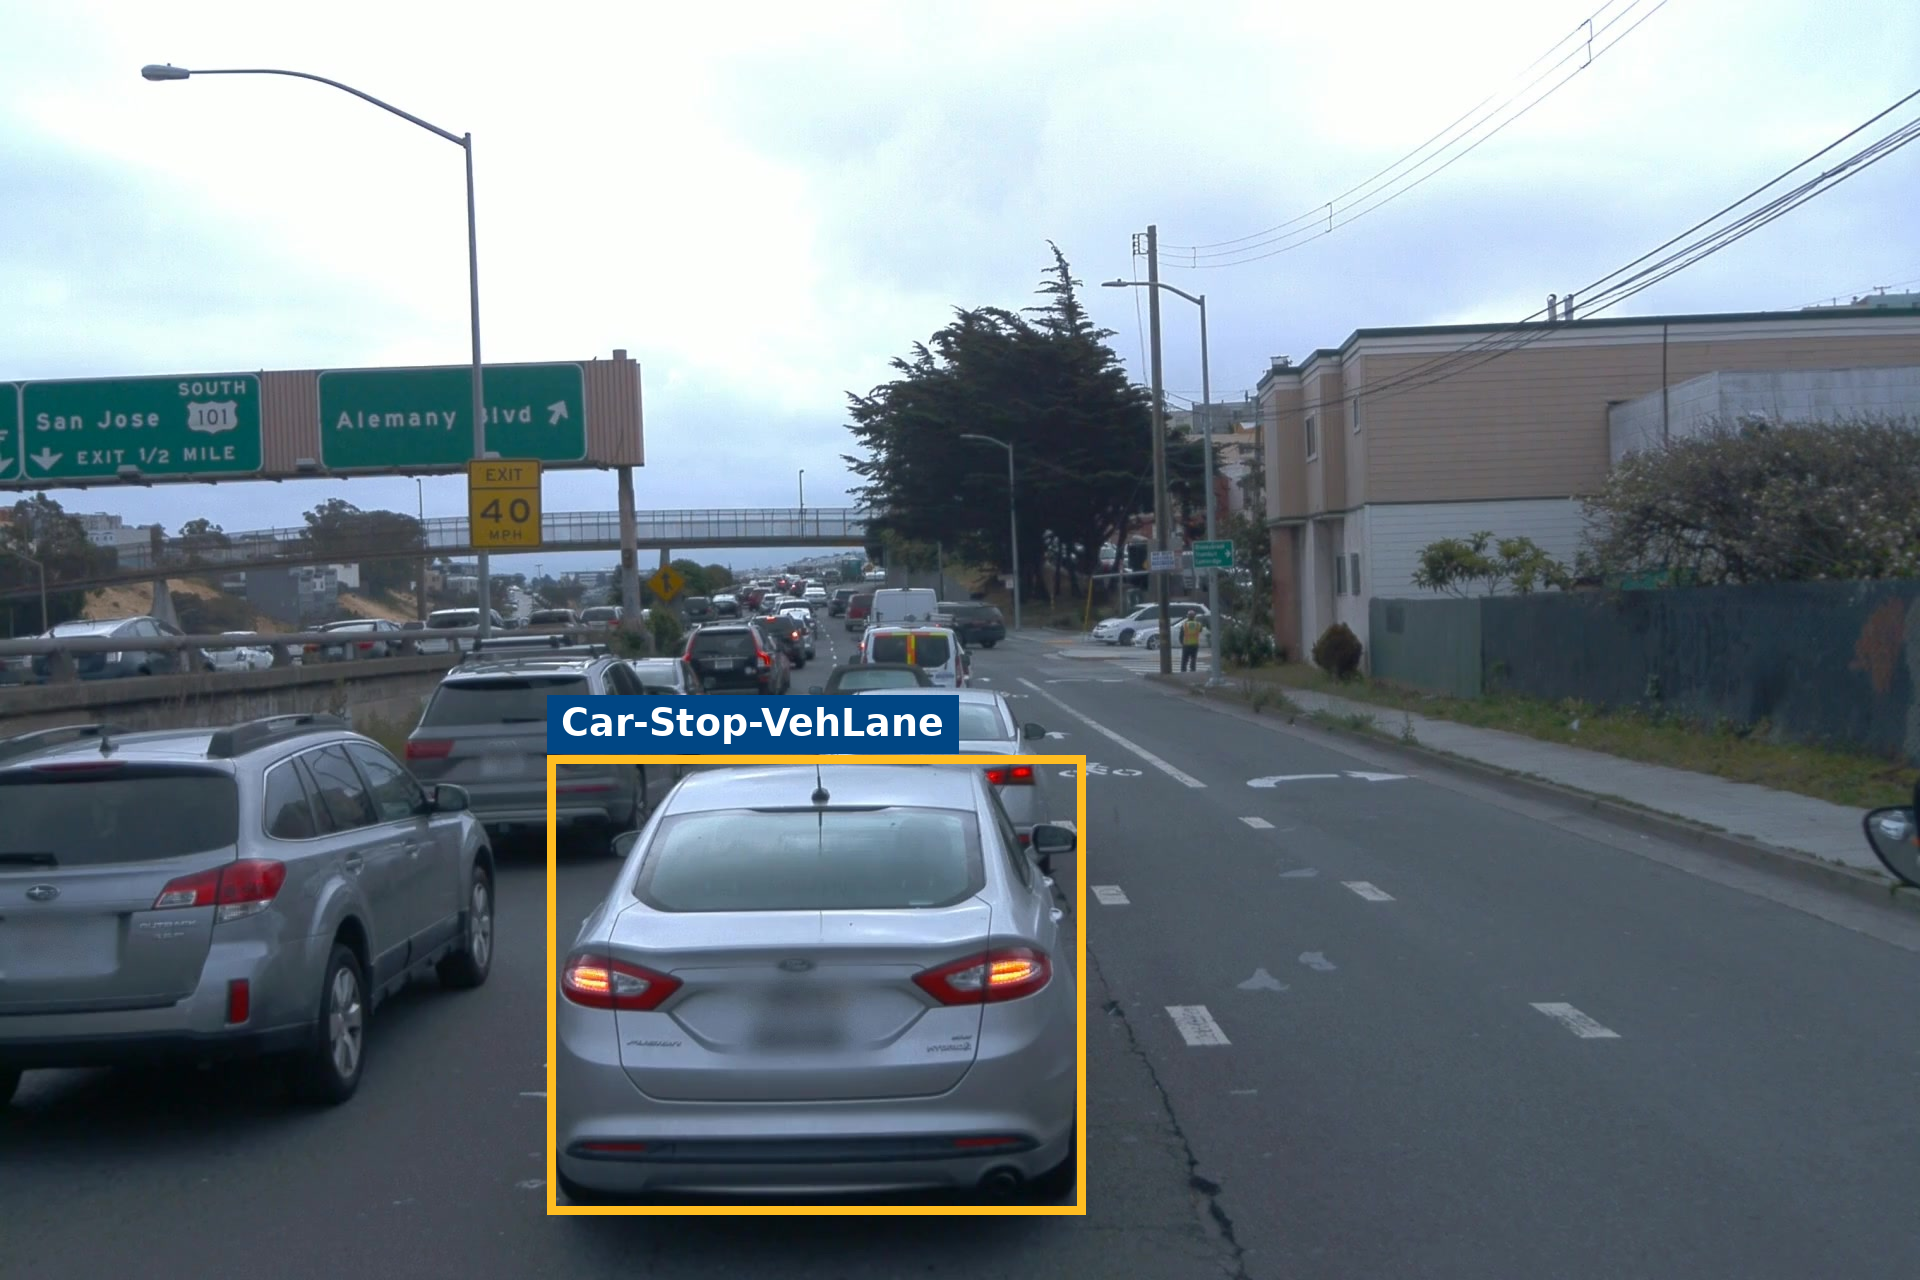
\includegraphics[width=0.88\textwidth,height=0.60\textheight,keepaspectratio]{Fig/road-event-example.png}
\caption[A labeled ROAD-Waymo road event.]{A labeled ROAD-Waymo road event \cite{road-waymo}. One ground-truth box is shown from video train\_00407, frame 00001, annotation b\_49; other boxes are omitted for clarity.}
\label{fig:road-event-example}
\end{figure}

The difficulty is that composition categories receive highly unequal training support. Common events contribute many examples, while a rare combination may have few labeled boxes even when its constituent agent or action is familiar. An overall mean can therefore conceal persistent weaknesses in rare-event recognition. Improving localization is useful, but it does not establish that a classifier can recognize the event associated with each newly detected object.

\section{Compositional Imbalance and the Research Problem}

The local training-count analysis covers 86 triplet classes. Counts range from 61 to 225,813 boxes, a ratio of approximately 3,702 to one. For class c with training count \(n_c\), define \(l_c = \log_{10}(n_c)\), \(\mu\) as the mean of those 86 log counts, and \(\sigma\) as their population standard deviation. The standardized value is \(z_c = (l_c - \mu)/\sigma\).

The geometric mean training count is \(10^\mu \approx 6{,}434\). The 47 classes with \(z < 0\) form the principal tail group. A nested deeper-tail group contains the 28 classes with \(z < -0.5\). The remaining 39 classes form the complementary common group. Membership depends only on training counts and stays fixed across model comparisons.

These groups are analytical definitions for this study, not claims that rarity measures driving risk. A rare label is not automatically more hazardous than a common one. The motivation is to make unequal recognition performance visible and test a mechanism that may help categories with limited training support.

\begin{figure}[htbp]
\centering
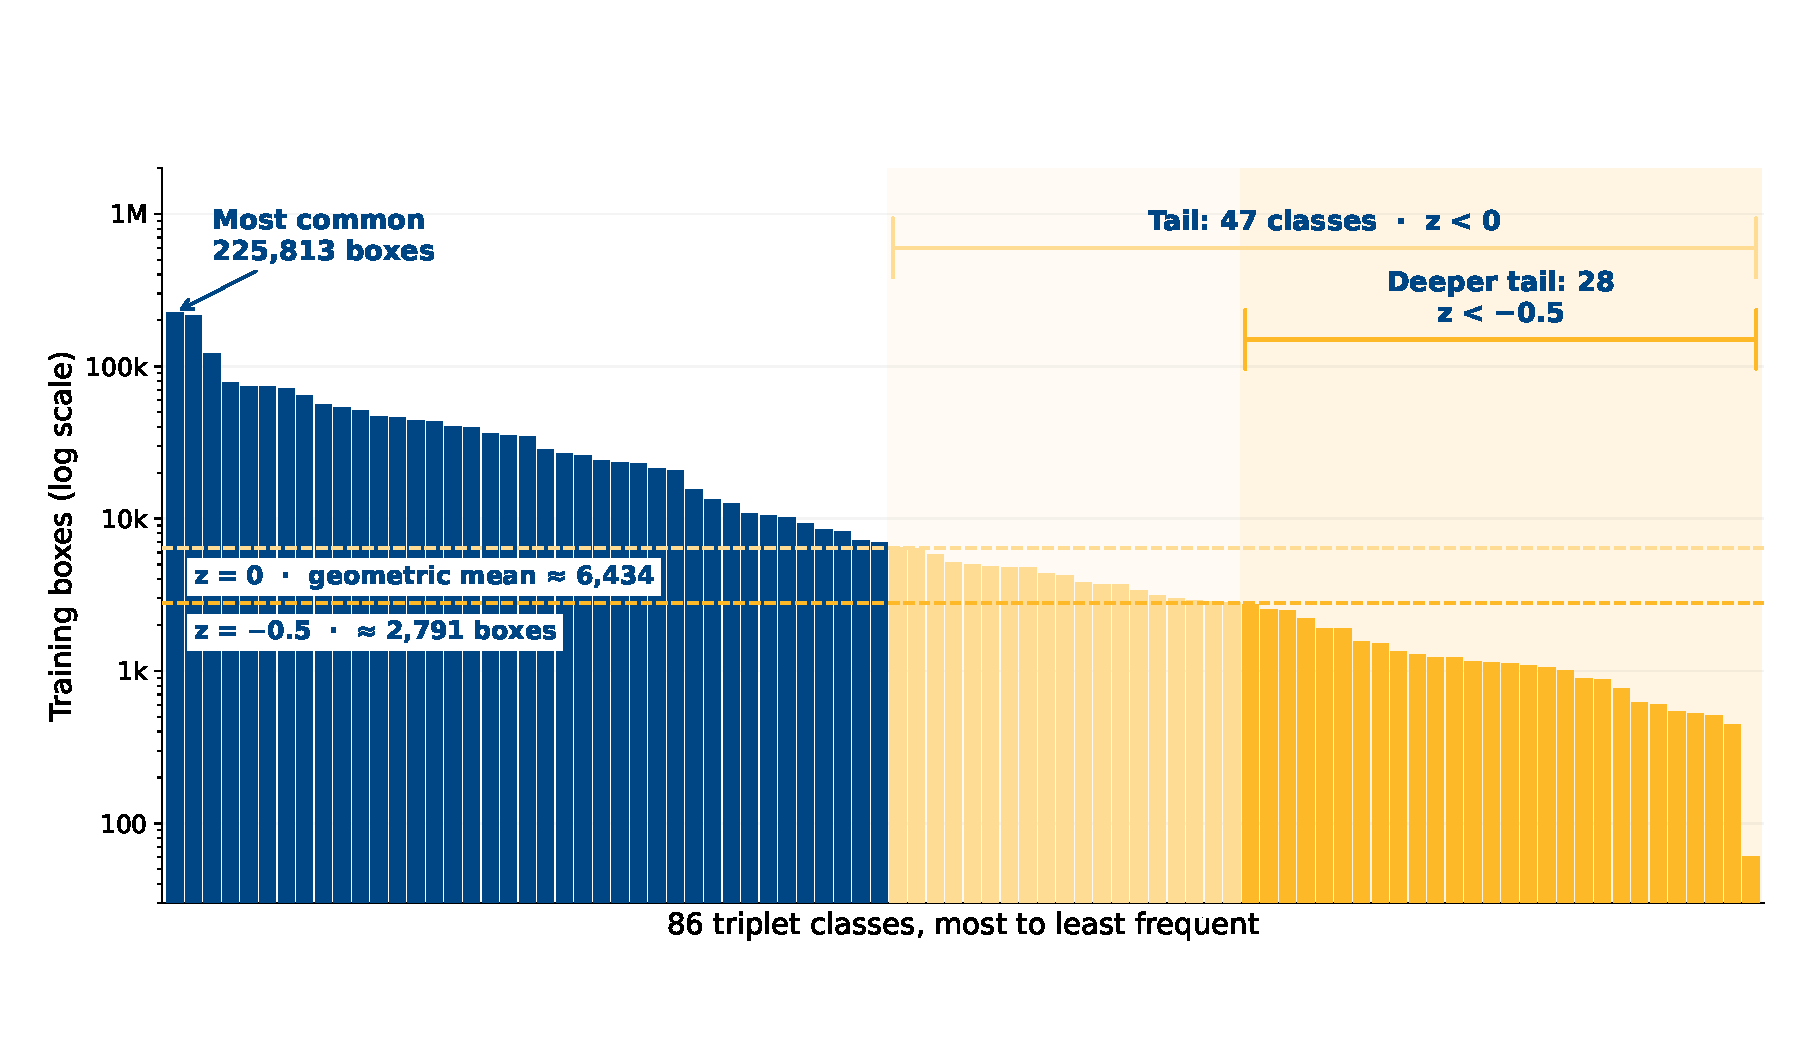
\includegraphics[width=\textwidth,height=0.68\textheight,keepaspectratio]{Fig/triplet-training-tail.pdf}
\caption{ROAD-Waymo triplet training counts and tail definitions.}
\label{fig:1}
\end{figure}

Figure~\ref{fig:1} shows the training-frequency imbalance and the nested evaluation groups. The z-score is computed on log counts: \(z < 0\) is equivalent to a count below the geometric mean, while \(z < -0.5\) identifies classes farther below it. These thresholds define evaluation populations; they do not assert that the counts follow a normal distribution.

\section{Research Objectives and Developed Approach}

The central question is whether rare road-event compositions can benefit from shared structural and semantic information without obscuring performance losses on common classes. The completed work asks how detector replacement, direct feature access, and learned composition change performance. The proposed work asks whether a phrase-based classifier contributes useful semantic structure when relevant visual inputs and evaluation conditions are controlled.

A related question concerns attribution: if the proposed system improves, is the gain associated with the crop representation, classifier design, or semantic directions? The study will qualify each claim using the comparisons that support it and will report cases where the evidence is mixed.

We have developed a decoupled pipeline to investigate these questions. A YOLOv8x detector supplies candidate boxes and agent identities. A frozen video backbone supplies regional appearance and motion features, and a trained linear classifier predicts actions, locations, and compositions. A stacked composition multilayer perceptron (MLP) then combines the primitive predictions with the visual feature to estimate duplex and triplet scores. This design separates finding an object from describing its event and allows the composition classifier to be changed while candidate boxes and primitive outputs remain fixed.

The experimental development begins with a replicated 3D-RetinaNet baseline. A detector-replacement comparison transfers its event scores to YOLO boxes through overlap matching; a subsequent comparison extracts features directly at every candidate box. These comparisons establish which changes concern localization, feature access, or composition learning. We refer to this completed sequence as Stages 0--3 when presenting the methods and results. The proposed extension, Stage 4, will connect frozen InternVideo2 crop features to text embeddings of benchmark event descriptions. It will test semantic classifier structure against controls using the same visual inputs and evaluation population.

\section{Contributions and Scope}

The completed contribution is a reproducible detector--classifier platform and a controlled learned-composition comparison. Under the shared-frame evaluation protocol, replacing independent composition outputs with the stacked MLP improves triplet f-mAP from 6.65\% to 9.73\%, while the earlier outputs remain fixed. The proposed contribution is to determine whether phrase-based classification can improve the remaining rare-composition gap, while reporting any losses on common classes.

The study evaluates frame-level detection within the fixed ROAD-Waymo vocabulary; deployment safety, causal intent prediction, and unseen-category generalization are outside its scope.

\chapter{Literature Review}

This thesis draws on research in road-event detection, long-tailed recognition, video representation learning, and vision--language classification. These areas address different parts of the problem: detecting an agent, representing its behavior, learning from unequal class frequencies, and sharing information among related event descriptions. The review distinguishes the evidence established in each setting from the questions that remain for rare ROAD-Waymo compositions. In particular, improvements in image classification, video recognition, or unseen attribute--object recognition are motivations for the proposed study, rather than direct evidence of improved road-event detection.

\section{Road-Event Benchmarks and Visual Representations}

Pedestrian-behavior research illustrates why detection alone is insufficient for scene understanding. JAAD pairs pedestrian boxes with behavioral and contextual annotations, enabling study of crossing behavior and interaction with traffic \cite{jaad-crossing}. PIE adds human-referenced crossing-intention estimation and future trajectory prediction \cite{pie}. These tasks connect appearance, motion, and context, but their targets must be distinguished: an observed crossing action, a future crossing outcome, and a human judgment of intention are different labels. ROAD extends the event-recognition setting across road-agent categories through agent, action, and location compositions. This thesis adopts that event vocabulary and does not transfer pedestrian-intention interpretations to ROAD-Waymo action labels.

Driving datasets differ in the relationships their annotations support. The Waymo Open Dataset provides synchronized camera and LiDAR observations with object annotations for perception research across varied locations \cite{waymo}. BDD100K supports heterogeneous driving tasks, including detection and other forms of scene understanding \cite{bdd}. These benchmarks establish the importance of localization and diverse observations, but object identity alone does not describe the event in which an agent participates. AVA offers a complementary action-detection setting: it associates spatially and temporally localized people with multiple atomic action labels \cite{ava}. Its relevance is the need to classify an actor within a scene rather than assign a single label to an entire video. Its movie-based action vocabulary and evaluation setting differ from those of road-event detection.

ROAD explicitly represents road events through agents, actions, locations, and their compositions. Singh et al. introduced the benchmark and a 3D-RetinaNet baseline for event detection \cite{road}. Duplex labels combine agent and action, while triplets also include location. ROAD-Waymo applies compatible event annotations to US driving video from Waymo Open, allowing comparison with the original UK ROAD data within the ROAD++ framework \cite{road-waymo}. The present thesis uses ROAD-Waymo rather than combining the two domains. Consequently, evidence about geographical transfer and evidence about rare compositions within ROAD-Waymo must remain separate.

ROAD-R adds explicit logical requirements to ROAD and studies learning and prediction mechanisms that use those requirements \cite{road-r}. This distinguishes two meanings of structure. Logical requirements specify which combinations are admissible; semantic representations describe similarities between class meanings. Encouraging constraint satisfaction during training is also different from enforcing admissibility at prediction time. A classifier may produce logically compatible outputs while failing to recognize the correct event. Conversely, improved average precision does not guarantee consistency between primitive and composition predictions. The proposed semantic classifier therefore addresses recognition and does not claim the guarantees of a constrained-output method.

The replicated detector connects several foundational visual architectures. Residual networks make deep representations easier to optimize through residual mappings \cite{resnet}. Inflated 3D networks extend image filters and pooling operations into the temporal dimension to learn video features \cite{i3d}. Feature Pyramid Networks combine a top-down pathway with lateral connections to obtain representations at several spatial scales \cite{fpn}. RetinaNet couples dense detection with focal loss, which reduces the training contribution of easy examples \cite{focal-loss}. ROAD's 3D-RetinaNet adapts this detection approach to road events \cite{road}. The local baseline uses a ResNet50-I3D backbone, so the I3D citation establishes the inflation principle without implying that the local model is the original paper's exact backbone.

Region features provide a basis for separating localization from classification. Mask R-CNN introduces RoIAlign to preserve spatial alignment when extracting a fixed-size representation for a region \cite{mask-rcnn}. In the developed pipeline, a detector supplies the box and RoIAlign reads a frozen video feature map at that box. This separates whether an object was proposed from what features are available to classify it. It also clarifies why copying scores from an overlapping detection is a different operation: score transfer remains dependent on the original detector producing a suitable match.

Video representations provide further alternatives to a fixed backbone. SlowFast networks use a slow pathway for spatial semantics and a faster pathway for fine temporal information \cite{slowfast}. Video Swin Transformer introduces local spatiotemporal attention through a hierarchical transformer design \cite{video-swin}. VideoMAE learns video representations by reconstructing heavily masked video content, emphasizing self-supervised pretraining \cite{videomae}. These approaches demonstrate that temporal sampling, architecture, and pretraining objectives can all influence the representation. They motivate controlling the visual input when evaluating semantic classifiers: replacing both an encoder and a classifier cannot isolate the effect of language-derived class structure.

\section{Learning Under Long-Tailed Class Distributions}

Class imbalance can affect both the representation and the decision rule learned from it. Focal loss addresses the dominance of easy examples in dense detection \cite{focal-loss}; this is related to, but not identical to, unequal support among foreground event categories. A rare triplet may remain difficult even after background examples receive less influence. Thus, the use of focal loss in the developed pipeline does not by itself establish that rare compositions have been adequately addressed.

Several approaches adjust how class frequency enters the learning objective. Cui et al. derive class-balanced weights from the effective number of samples, reflecting diminishing additional information as the number of examples grows \cite{class-balanced}. Cao et al. introduce a label-distribution-aware margin and defer reweighting until after an initial representation-learning period \cite{ldam}. Both methods use class frequency, but they intervene differently: one changes the contribution of examples, while the other changes class-dependent margins and the training schedule. For the proposed study, these distinctions reinforce the need to define tail membership from training data and to keep that definition fixed during evaluation.

Balanced Meta-Softmax addresses distribution shift between training and evaluation through Balanced Softmax and a complementary sampling mechanism \cite{balanced-softmax}. Menon et al. study frequency-based logit adjustment either after training or within the loss \cite{logit-adjust}. These methods show why a change in class scores may improve a class-balanced metric without changing the underlying features. Their softmax formulations also assume a multiclass setting that differs from the independent sigmoid outputs used for multi-label road events. Applying their conclusions directly to the proposed classifier would require an appropriate multi-label formulation and a separate experiment.

Decoupling offers an experimental way to study these effects. Kang et al. separate representation learning from classifier learning and show that adjusting a classifier over a naturally sampled representation can be effective on long-tailed image benchmarks \cite{decoupling}. BBN uses separate branches and a cumulative learning schedule to balance representation and classifier learning \cite{bbn}. These studies motivate treating the classifier as an explicit component rather than attributing every change to the encoder. The developed road-event pipeline follows this principle through frozen features and separately trained heads, while recognizing that image-level classification and box-level event detection have different supervision and error sources.

Other methods change representation geometry or model diversity. RIDE uses multiple distribution-aware experts to address bias and variance under long-tailed sampling \cite{ride}. Parametric Contrastive Learning introduces learnable class centers to counter the tendency of supervised contrastive learning to favor frequent classes \cite{paco}. These approaches show that shared structure can be imposed through more than language. A semantic classifier should therefore be assessed against a meaningful classifier control, rather than compared only with a weak independent-label baseline. They also motivate reporting common-class behavior, since improvements for rare categories may be accompanied by regressions elsewhere.

VL-LTR is especially relevant because it introduces class-level text descriptions into long-tailed visual recognition \cite{vl-ltr}. It learns visual and linguistic representations and reports benefits for classes with fewer image examples. This provides evidence that language can contribute to recognition under imbalance, but it does not establish the same outcome for multi-label road-event boxes. The proposed study differs in using a fixed benchmark vocabulary, frozen crop features, and fixed phrase embeddings with a supervised projection. Its evaluation must establish whether those design choices help rare triplets under the road-event protocol.

Taken together, these methods identify several possible explanations for a tail improvement: better visual features, changes in sampling or loss, classifier calibration, additional capacity, and information shared among classes. The thesis focuses on learned composition and semantic classifier directions. Frequency-based methods remain relevant alternatives, while the primary ablations are designed to distinguish semantic structure from changes to the representation and classifier.

\section{Vision--Language Adaptation for Video Recognition}

CLIP learns aligned image and text representations through contrastive pretraining, allowing class descriptions to define classifier directions \cite{clip}. The resulting relationship between language and visual content is the basis for considering event phrases as more informative than unrelated class identifiers. However, a description that is linguistically plausible may not distinguish visually similar actions or locations. The relevant question is whether the learned alignment retains the distinctions needed for road-event recognition.

Prompt-learning methods demonstrate both the usefulness and sensitivity of text-based classification. CoOp learns context vectors while keeping the pretrained model fixed \cite{coop}. CoCoOp conditions part of the prompt on the input to improve generalization beyond the classes used for adaptation \cite{cocoop}. MaPLe couples prompts in the visual and language branches to adapt their representations together \cite{maple}. These methods make different parts of the model trainable. They therefore cannot be treated as equivalent to a classifier whose phrase matrix remains frozen. For this proposal, their main implication is that the choice and adaptation of class descriptions must be documented and controlled.

Adaptation can also use labeled visual examples directly. Tip-Adapter builds a key--value cache from a few-shot training set and combines feature retrieval with the pretrained model's predictions \cite{tip-adapter}. It provides a useful contrast to prompt learning: downstream performance may improve through visual evidence without changing the textual description. This motivates keeping the training population and feature source fixed when comparing the proposed semantic head with a free classifier. A difference between those heads can then be interpreted more narrowly than a comparison in which the representations and examples also change.

Transferring image--text models to video introduces temporal design choices. X-CLIP uses cross-frame attention and video-dependent prompting to adapt pretrained image--language representations to video recognition \cite{xclip}. Ju et al. combine continuous prompts with lightweight temporal transformers over frame features \cite{efficient-prompt}. ViFi-CLIP shows that fine-tuning and pooling frame-level CLIP features can provide a strong video baseline without requiring a complex new temporal module \cite{vifi}. Together, these studies caution against attributing an improvement to semantic reasoning merely because a vision--language model is involved. Temporal processing, adaptation, and pooling can each contribute.

InternVideo2 develops a family of video models through progressive training that combines masked video modeling, cross-modal contrastive learning, and generative objectives \cite{internvideo2}. The proposed implementation uses the released InternVideo2\_CLIP\_S model, whose repository supplies its configuration and weights \cite{internvideo2-clip-s}. The family-level paper motivates the representation, while the model release identifies the specific component used in this thesis. The proposed head reads an internal crop descriptor and learns a projection into the phrase space; it does not assume that the internal descriptor is already the released model's final video--text embedding.

The distinction between pretraining and the proposed experiment is central. Contrastive video--text learning has already shaped the frozen encoders. The planned ROAD-Waymo experiment instead trains a supervised classifier using those representations. It tests whether retaining semantic directions is useful for rare benchmark compositions. It does not claim that the supervised head itself performs new contrastive pretraining, or that the presence of text automatically provides temporal reasoning.

\section{Compositional Structure and the Research Gap}

Compositional recognition asks how predictions for parts relate to predictions for their combinations. ROAD considers both direct composite prediction and composition of primitive scores \cite{road}. The developed MLP follows the former goal through a structured input: it receives primitive predictions together with visual features and learns scores for the benchmark's valid duplexes and triplets. This gives it access to relationships that a fixed product or minimum of primitive scores cannot adapt to the task. It does not impose logical agreement between independently predicted heads.

Compositional zero-shot learning provides related evidence about sharing information among concepts. Naeem et al. connect states, objects, and their compositions through a graph so that relationships among primitives inform composition classifiers \cite{cge}. Nayak et al. learn compositional soft prompts in which attribute and object tokens can be recombined to describe unseen combinations \cite{csp}. These methods explicitly target generalization to compositions absent during training. The proposed ROAD-Waymo study instead evaluates a fixed vocabulary that includes rare but observed classes. Their results motivate structured sharing, but do not justify a zero-shot claim for this thesis.

The literature therefore supports a focused gap rather than the claim that semantic classification is new in general. Long-tailed recognition studies frequency-sensitive losses, decoupled classifiers, and linguistic information; video adaptation studies the transfer of image--text representations; compositional learning studies shared primitives and combinations. What remains to be established here is whether fixed phrase-based classifier directions improve rare ROAD-Waymo triplets when the visual inputs, candidate boxes, training examples, and evaluation population are controlled.

The developed pipeline supplies the comparison platform. The proposed experiments will relate tail AP to overall and common-class AP, inspect per-class changes, and repeat classifier training with recorded seeds. A positive result must be supported by the relevant ablations, while a negative result can identify limitations in the visual evidence or its alignment with event descriptions. This framing connects the related work to an empirical question that the proposed experiment can answer without assuming that semantic structure will necessarily help.

\chapter{Methodology}

We developed the ROAD-Waymo pipeline through controlled changes to a replicated joint detector. Detector replacement and score transfer are followed by direct region-feature classification and learned composition. This chapter defines these completed methods and their shared evaluation protocol. The resulting rare-composition gap motivates the semantic-classifier study in Chapter 5.

The completed stages share the benchmark label layout and evaluator. Changes in boxes, representation, classifier, and composition are described explicitly so that improvements are attributed only to the intervention supported by a comparison.

\section{Dataset, Prediction Targets, and Evaluation}

The study uses the ROAD-Waymo training and validation partitions \cite{road-waymo}: 600 training videos and 198 validation videos. The publicly unannotated test partition is outside the reported evaluation. Dataset counts and tail membership refer to the local annotation release and project audit, rather than substituting aggregate counts reported for other releases.

Each candidate is associated with the score groups in Table~\ref{tab:2}. Agentness is a separate object-presence score. Action and location are multi-label tasks, and each composition is a benchmark-defined combination. The total is 1 + 10 + 22 + 16 + 49 + 86 = 184.

\begin{table}[htbp]
\centering
\caption{Prediction groups and output dimensions.}
\label{tab:2}
\begin{singlespace}
\begin{tabular}{@{}lcc@{}}
\toprule
\textbf{Prediction groups} & \textbf{Dimensions} & \textbf{Meaning} \\
\midrule
Agentness + agent & 1 + 10 & Presence + identity \\
Action + location & 22 + 16 & Activity + position \\
Duplex + triplet & 49 + 86 & Event compositions \\
Total & 184 & Six output groups \\
\bottomrule
\end{tabular}
\end{singlespace}
\end{table}

All completed-stage comparisons use frame-level mean average precision at IoU 0.5 through the baseline repository’s evaluator. Predictions are ranked by class and matched to ground truth on each frame. AP summarizes the precision--recall curve; mAP averages class APs. The reported comparison is restricted to 36,717 validation frames shared by the detection sources and required feature records.

Figure~\ref{fig:frame-map} shows how a scored box contributes to this metric. For each class, the evaluator processes detections in descending score order within a frame and matches each detection to an available ground-truth box of that class when IoU is at least 0.5. Each ground-truth box can be matched once. Unmatched detections, including duplicate detections after a ground-truth box has been consumed, count as false positives. The evaluator then ranks detections across the selected frames to obtain a precision--recall curve. It integrates the interpolated precision envelope at changes in recall and averages AP over the classes in the reported group. This follows the detection-evaluation principles of PASCAL VOC \cite{voc}; the actual implementation is the ROAD baseline evaluator \cite{road}.

\begin{figure}[htbp]
\centering
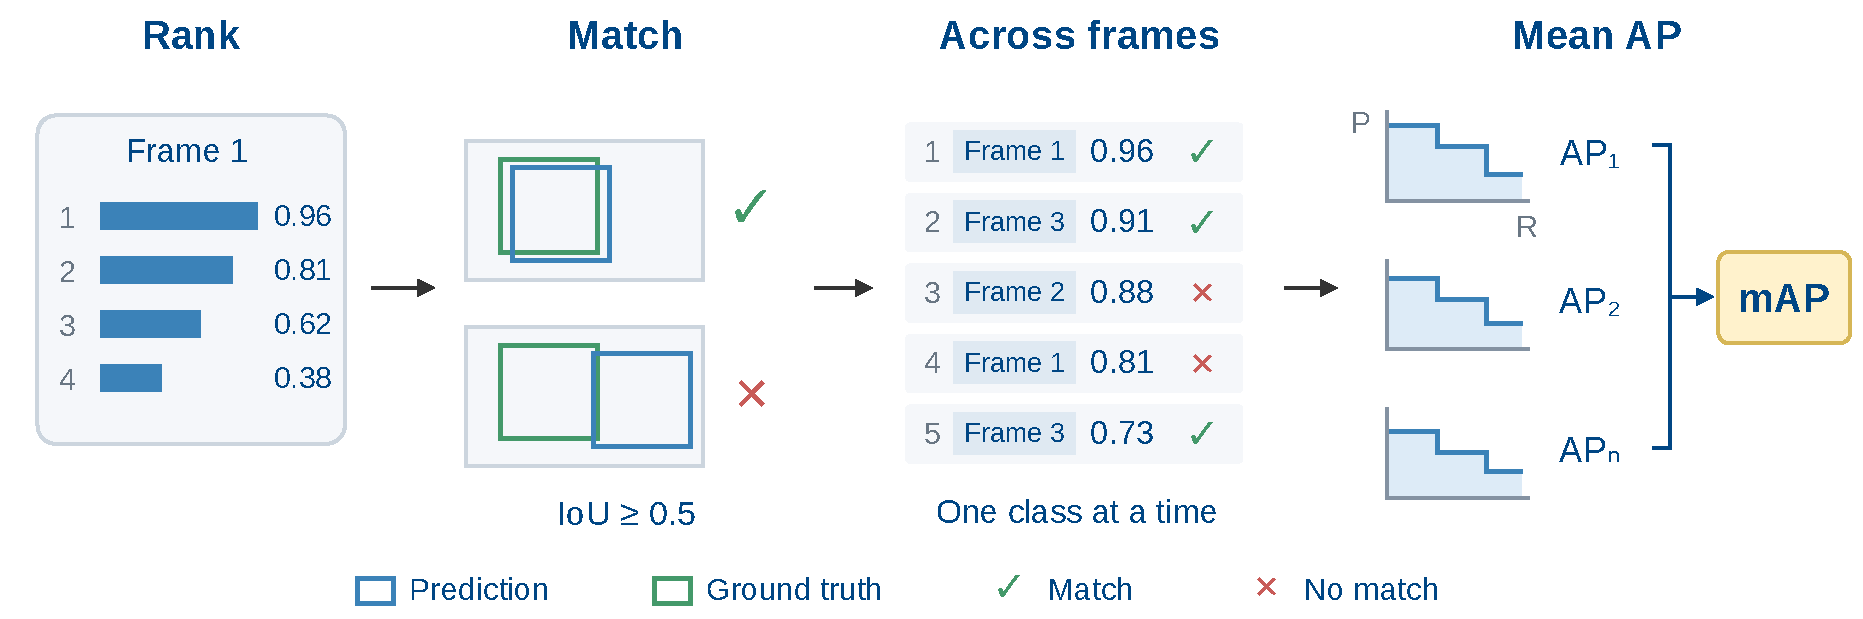
\includegraphics[width=\textwidth,height=0.60\textheight,keepaspectratio]{Fig/frame-map.pdf}
\caption[Frame-level average-precision evaluation.]{Frame-level average-precision evaluation. Scores and curves are schematic; matching is class-specific and restricted to the same frame.}
\label{fig:frame-map}
\end{figure}

“Full-candidate” denotes a broad low-threshold candidate pool, capped at 300 per frame, rather than exhaustive boxes or every annotated validation frame. Stage 0 uses its own candidates. Stages 1--3 share YOLO candidates. The original baseline validation path filters scores per class and per frame; the comparison path assembles predictions from saved dumps, including temporally averaged agentness for baseline candidate selection. Thus, using the same metric code alone does not make different filtering protocols equivalent.

The primary metric is f-mAP, not tube-level video-mAP. No test-server result is claimed. Training labels define tail membership, while validation predictions determine AP. The same tail class lists are used for every compared model.

\section{Replicated Joint Baseline}

The starting point is 3D-RetinaNet, which processes eight-frame clips through an I3D backbone and feature pyramid before predicting box offsets and class scores \cite{road}. Localization and classification share a learned representation. The replicated checkpoint provides both the baseline detections and the frozen visual backbone used in the early hybrid stages.

Two evaluations are distinguished. The earlier baseline validation produced 17.76\% agent and 9.17\% triplet f-mAP. The Stage 0 row in this proposal’s shared-frame comparison is 16.67\% agent and 7.54\% triplet f-mAP. The difference reflects evaluation conditions, including frame selection and candidate filtering; the numbers are not interchangeable.

Figure~\ref{fig:2} gives the Stage 0 data flow. The trained baseline predicts its own boxes and event scores; later hybrid stages reuse its frozen backbone or detections.

\begin{figure}[htbp]
\centering
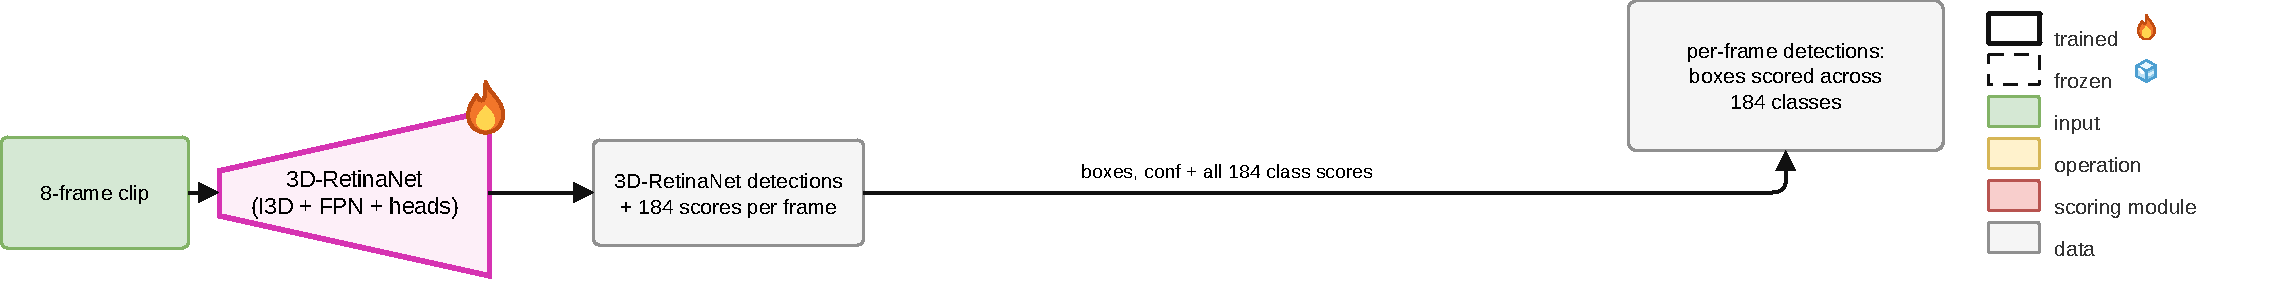
\includegraphics[width=\textwidth,height=0.68\textheight,keepaspectratio]{Fig/stage0-baseline.pdf}
\caption{Stage 0 joint detection and classification baseline.}
\label{fig:2}
\end{figure}

Figure~\ref{fig:3} details the ResNet50-I3D feature pyramid and detection subnets in the replicated 3D-RetinaNet. RetinaNet introduced focal loss for dense one-stage detection \cite{focal-loss}; ROAD adapts this architecture to video road-event detection \cite{road}.

\begin{figure}[htbp]
\centering
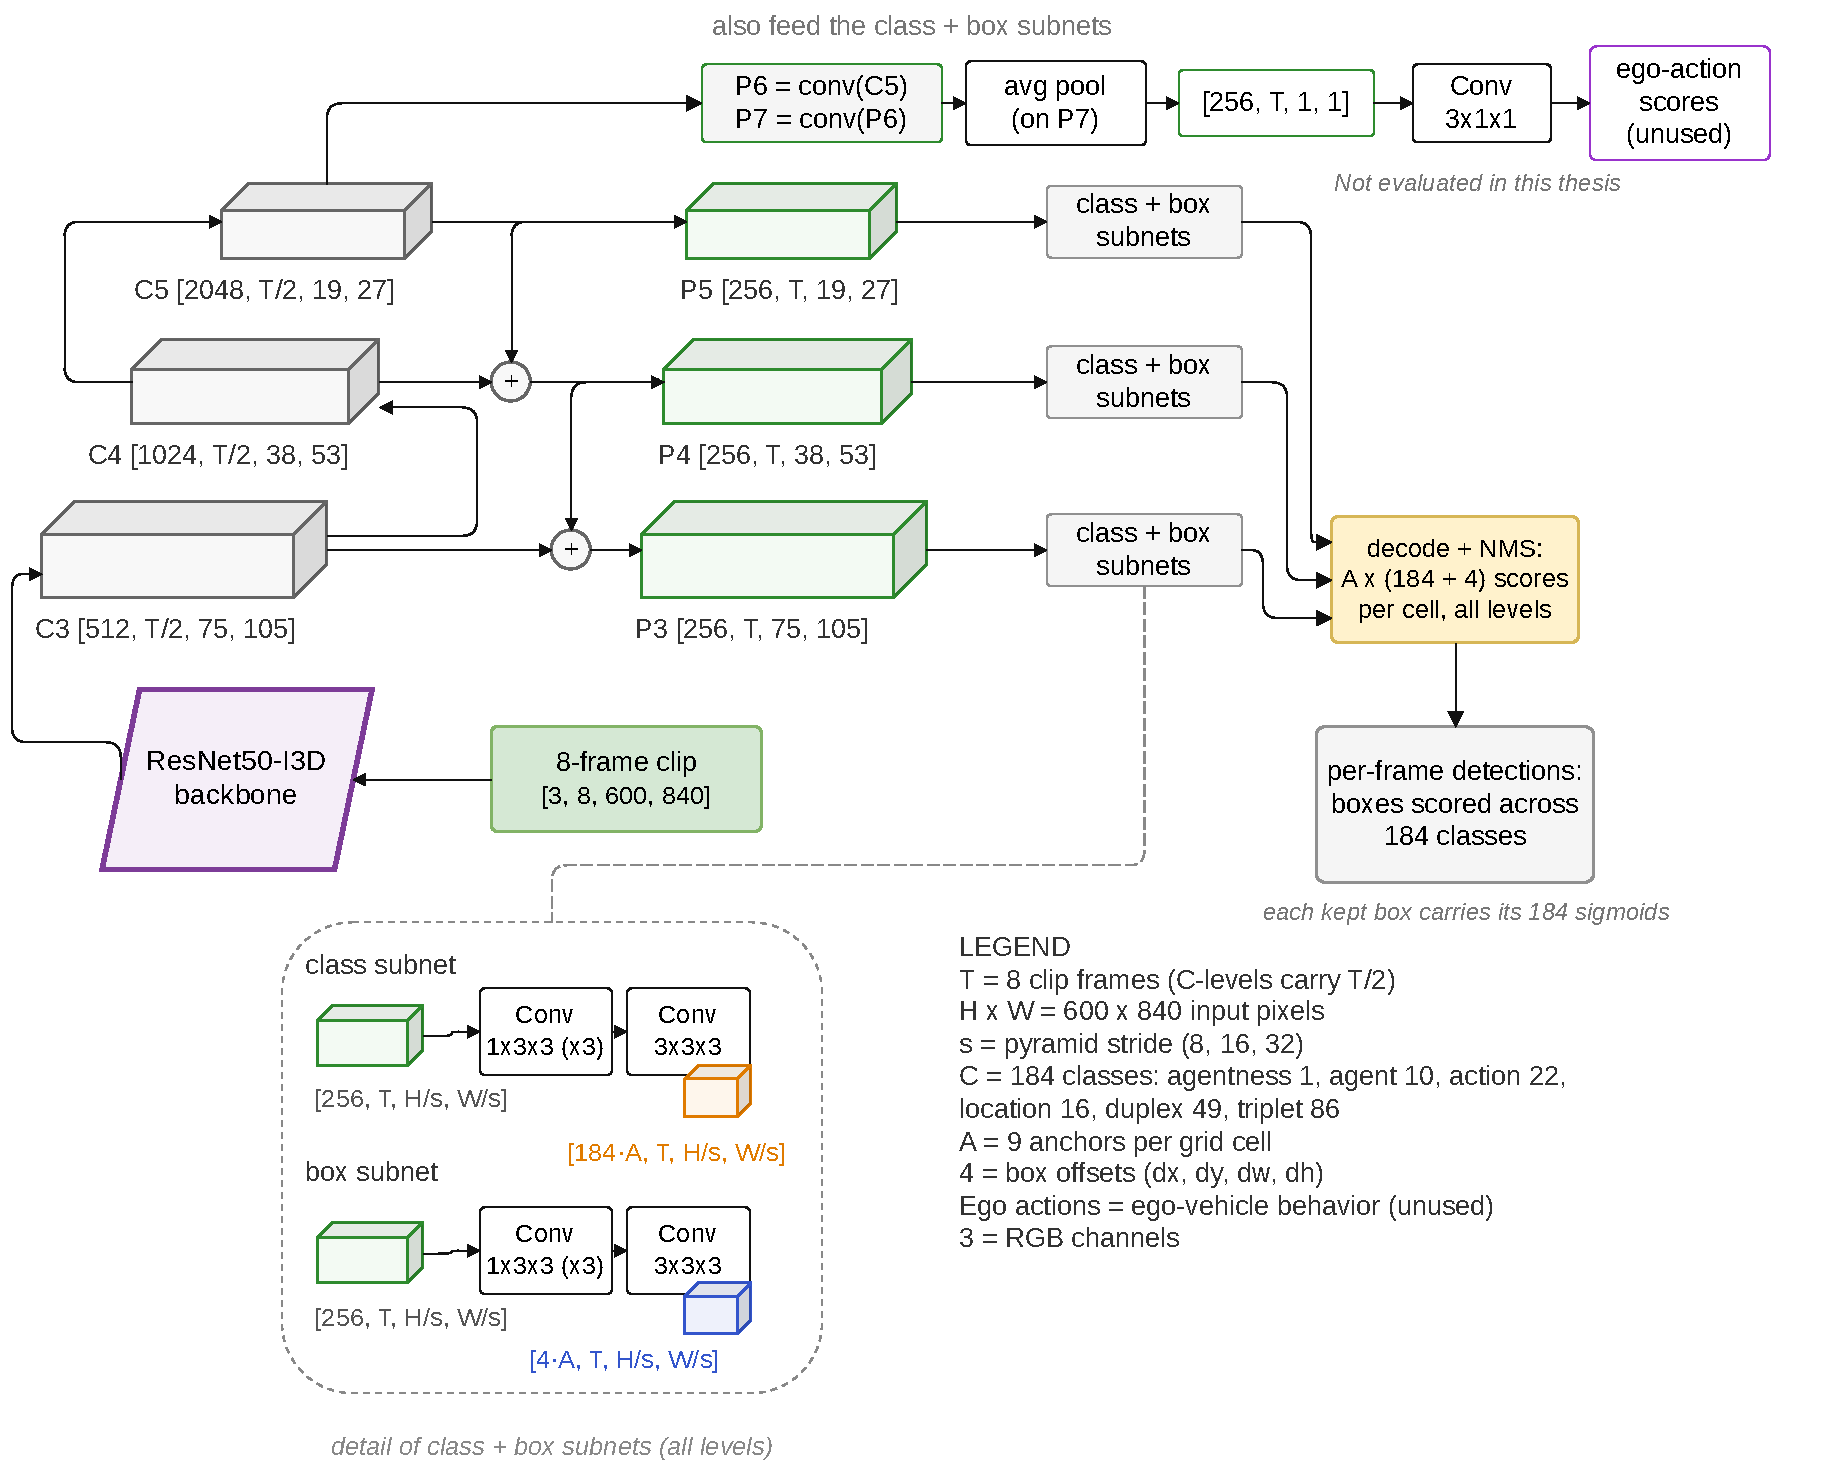
\includegraphics[width=\textwidth,height=0.68\textheight,keepaspectratio]{Fig/retinanet3d.pdf}
\caption{Replicated 3D-RetinaNet with a ResNet50-I3D backbone and feature pyramid.}
\label{fig:3}
\end{figure}

\section{Detector Replacement and Score Transfer}

YOLOv8x \cite{yolov8}, fine-tuned on ROAD-Waymo agent classes with a 1280-pixel input setting, supplies candidate boxes, confidence, and hard agent identity. The project training configuration follows the ECCV 2024 Track-1 recipe with documented implementation choices; the selected checkpoint is the recorded epoch-1 model. Candidate generation uses confidence 0.001, NMS IoU 0.7, and at most 300 detections per frame.

Figure~\ref{fig:4} details the YOLOv8x detector used for agent localization. The 1280 \(\times\) 1920 annotation identifies source-frame dimensions; the implementation applies Ultralytics resizing and letterboxing with imgsz = 1280. The 50-epoch setting describes the configured training recipe, while the reported comparison uses the selected epoch-1 checkpoint.

\begin{figure}[htbp]
\centering
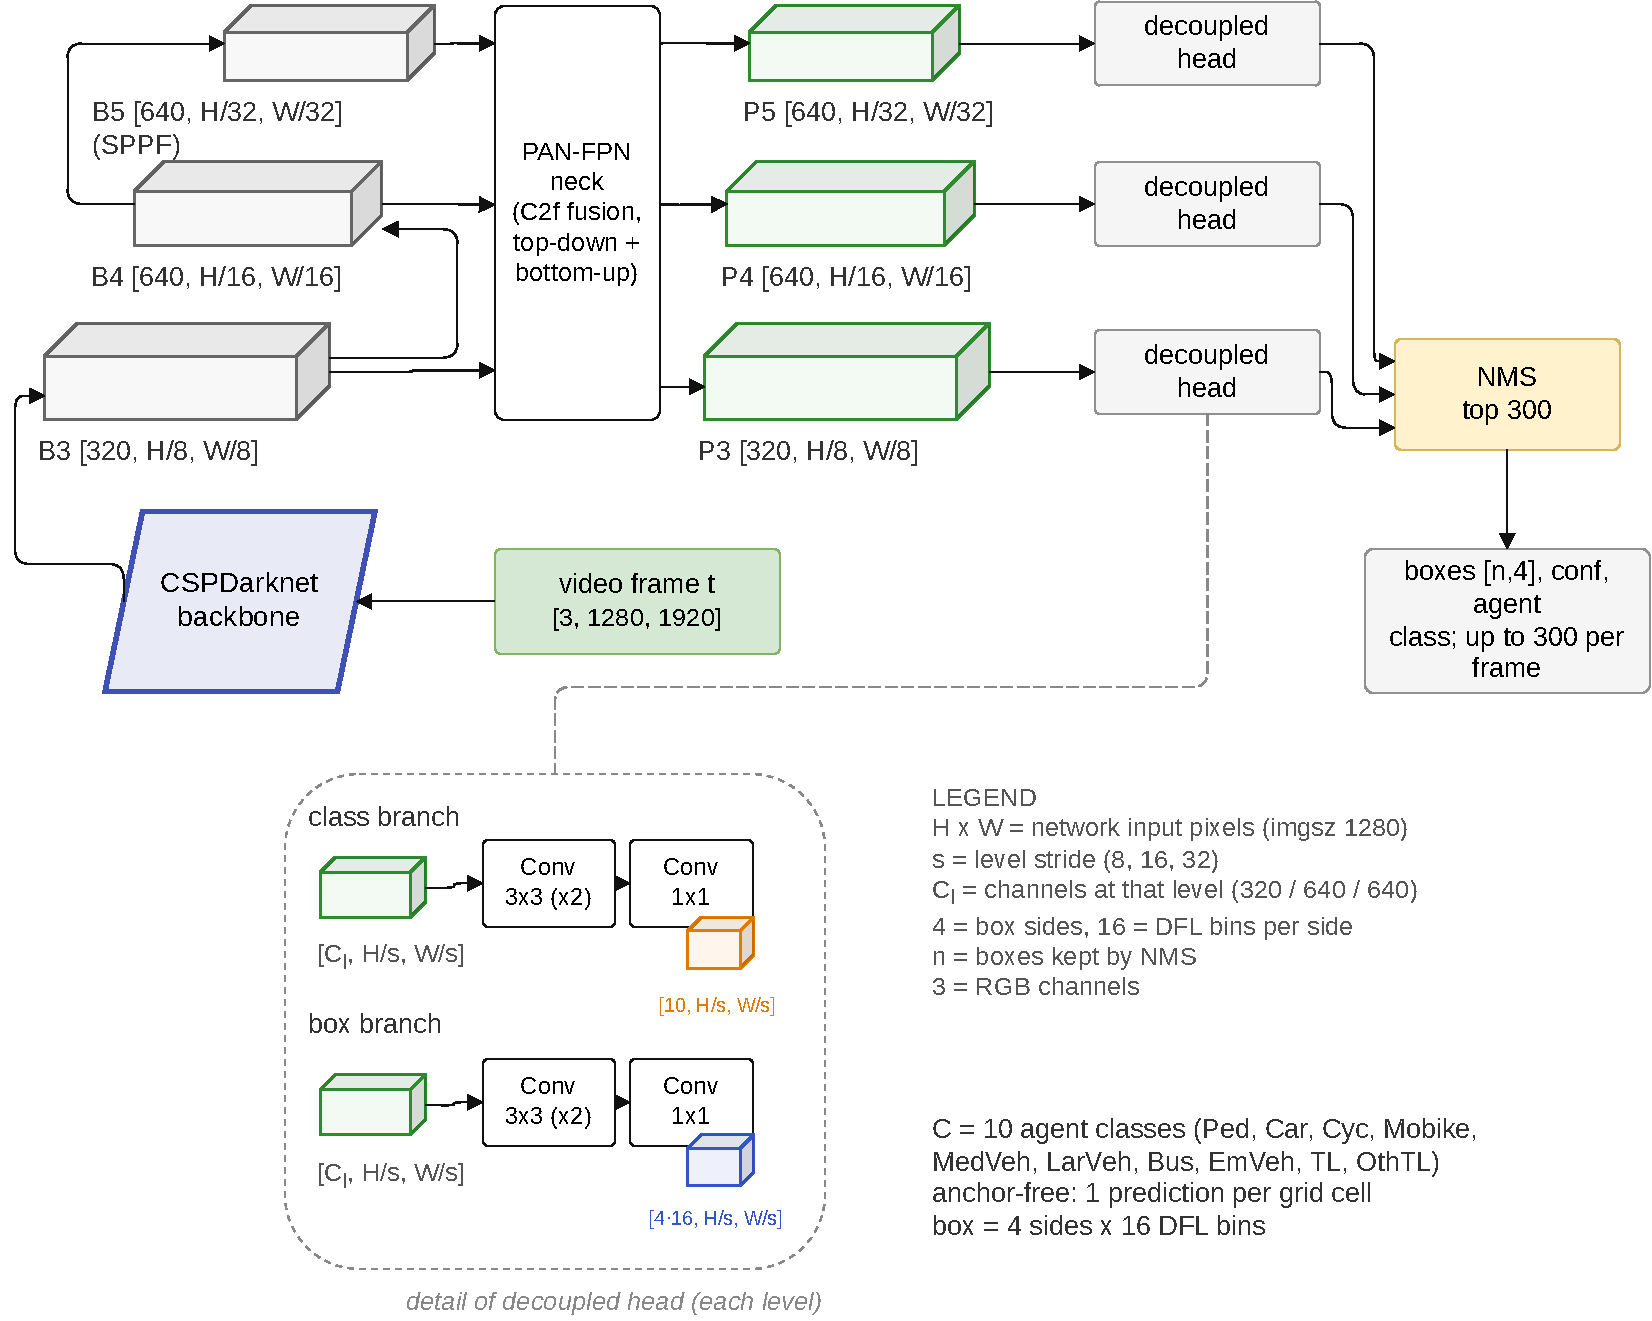
\includegraphics[width=\textwidth,height=0.68\textheight,keepaspectratio]{Fig/yolov8x.pdf}
\caption{YOLOv8x agent-detector architecture.}
\label{fig:4}
\end{figure}

For each YOLO box, Stage 1 finds the baseline detection with highest IoU on the same frame. If IoU is at least 0.5, the action, location, duplex, and triplet scores are copied from that detection. Otherwise, those scores remain zero. Matching is performed independently per YOLO box and does not impose a one-to-one assignment. YOLO supplies the emitted agentness and agent-class detections. No new score-transfer module is trained. Transferred event scores are emitted directly, without multiplication by YOLO confidence.

Across the 36,717 shared frames, approximately 40.6\% of 6,163,968 YOLO candidates find a qualifying baseline match. This is the proportion of candidates that receive transferred event scores; it is not ground-truth recall or classification accuracy. Figure~\ref{fig:score-transfer-limit} illustrates why: an unmatched YOLO box has no baseline event-score source, so its transferred action, location, duplex, and triplet values remain zero. A correctly localized object can consequently lack useful event predictions. The next stage addresses this dependence by extracting a feature at every candidate box.

\begin{figure}[htbp]
\centering
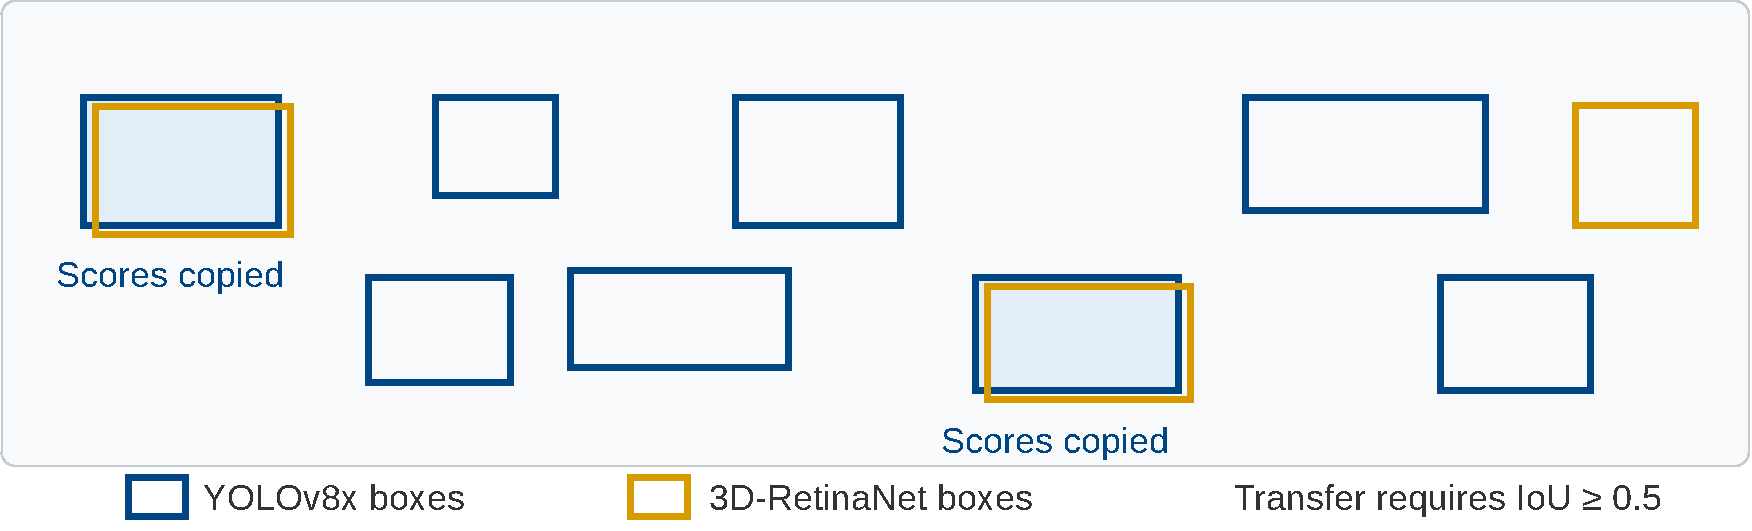
\includegraphics[width=\textwidth,height=0.60\textheight,keepaspectratio]{Fig/score-transfer-limit.pdf}
\caption[The event-score coverage limitation of overlap transfer.]{The event-score coverage limitation of overlap transfer. The boxes illustrate matched and unmatched candidates; their counts do not represent the measured match rate.}
\label{fig:score-transfer-limit}
\end{figure}

Figure~\ref{fig:5} summarizes the score-transfer path: overlap matching determines whether a YOLO candidate receives the baseline’s event scores.

\begin{figure}[htbp]
\centering
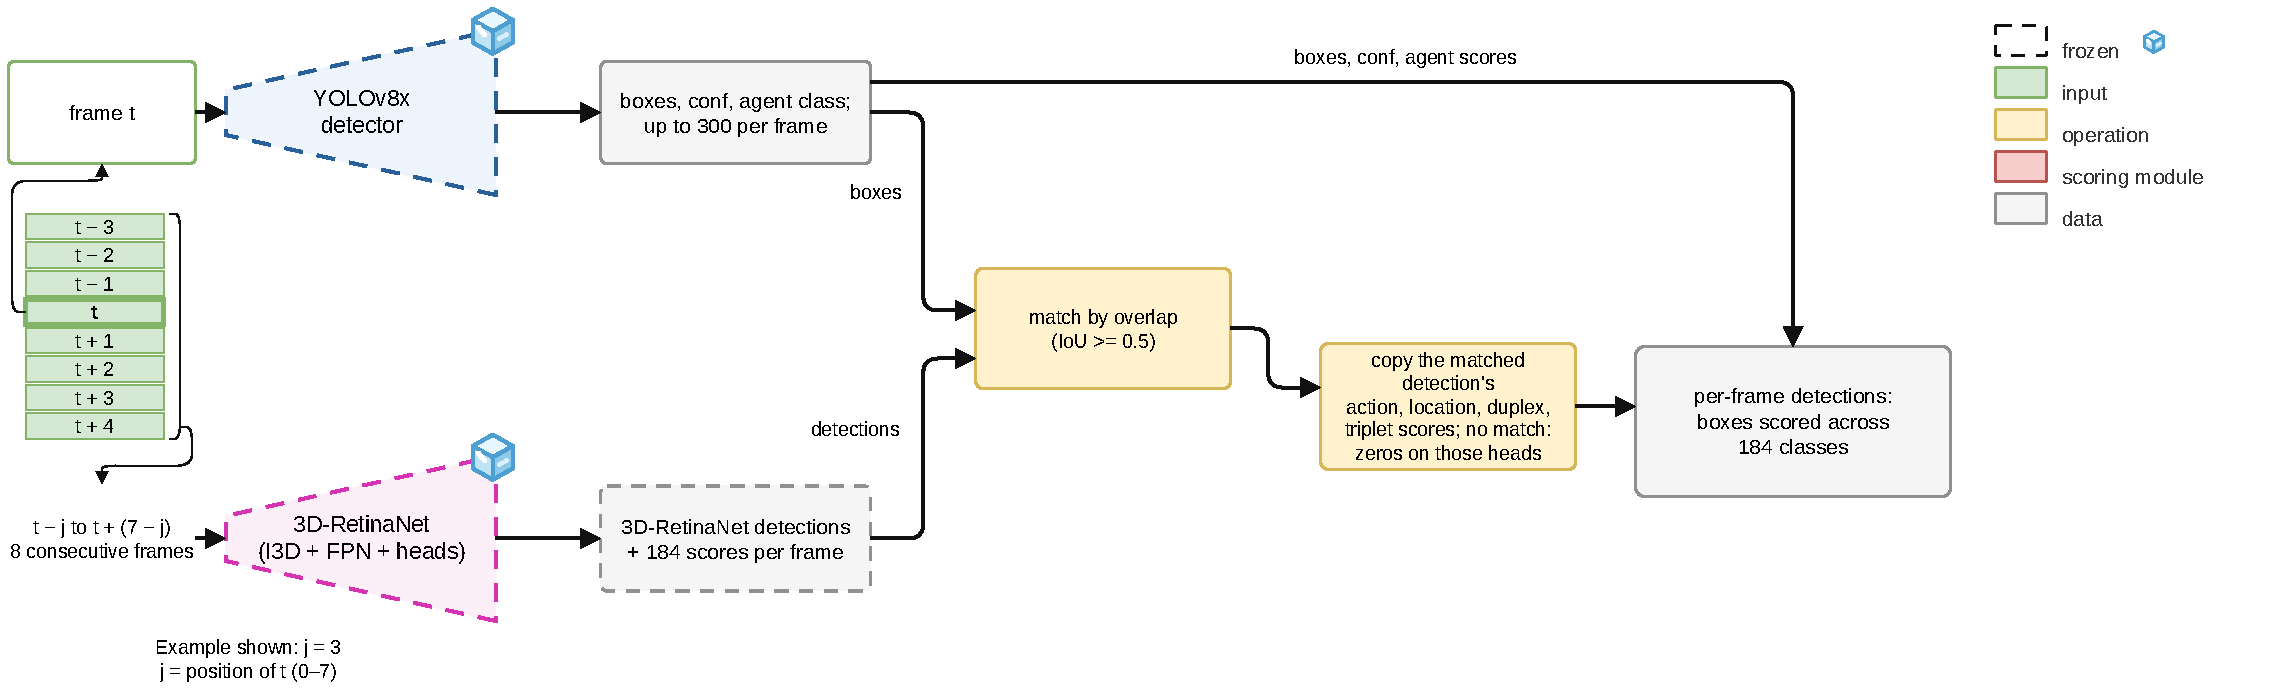
\includegraphics[width=\textwidth,height=0.68\textheight,keepaspectratio]{Fig/stage1-transfer.pdf}
\caption{Stage 1 detector replacement and overlap-based score transfer.}
\label{fig:5}
\end{figure}

\section{Direct Region Features and Event Classification}

Stage 2 replaces overlap-based score transfer with feature extraction at each YOLO box. Figure~\ref{fig:stage2-roialign} shows the detector--classifier path: the detector and video backbone remain frozen while the event head is trained.

\begin{figure}[htbp]
\centering
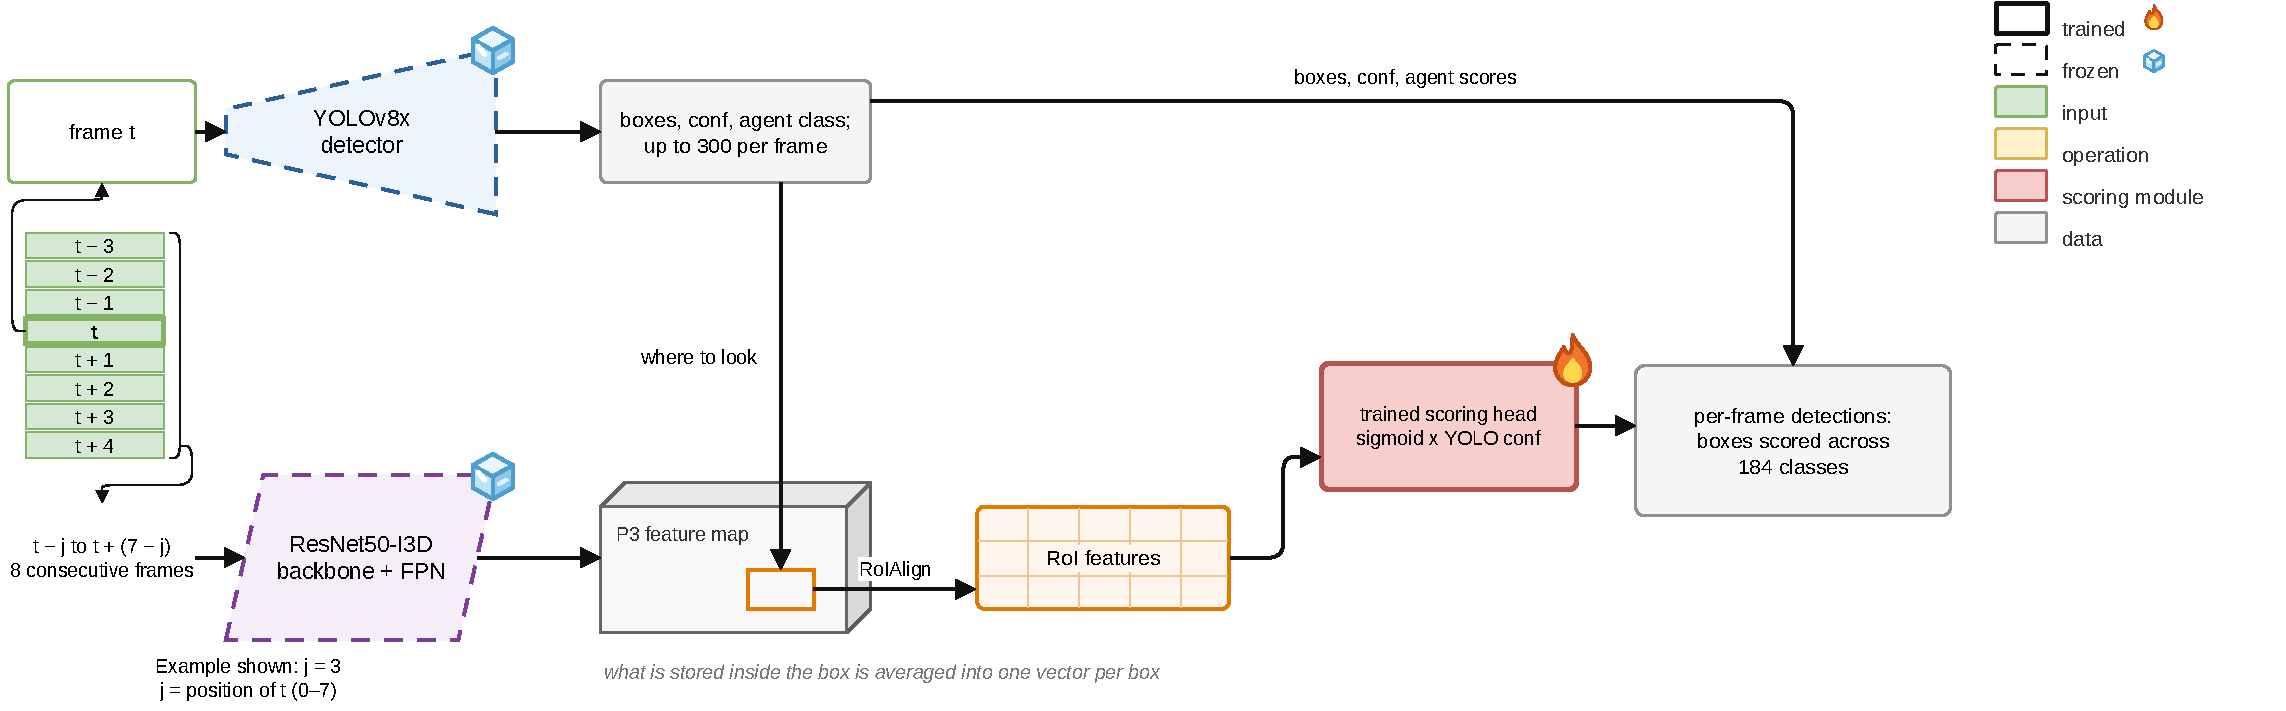
\includegraphics[width=\textwidth,height=0.60\textheight,keepaspectratio]{Fig/stage2-roialign.pdf}
\caption[Stage 2 direct region-feature classification.]{Stage 2 direct region-feature classification.}
\label{fig:stage2-roialign}
\end{figure}

Stage 2 reads the frozen I3D/FPN P3 feature map at every YOLO box using RoIAlign \cite{mask-rcnn}. Boxes are mapped into feature-map coordinates and pooled to one 256-dimensional vector at the corresponding frame. Temporal interpolation aligns the feature map with the clip length when needed. Unlike score transfer, this procedure can obtain a feature at a location that the baseline detection head did not select.

Figure~\ref{fig:roi-align} expands this operation. The implementation rescales box coordinates to the P3 grid, selects the feature slice for the target frame, and applies aligned RoIAlign with a single spatial output bin. Bilinear sampling and averaging produce one 256-dimensional vector for each box. The illustrated sample locations explain the pooling operation; they are not additional detections. Because the map was produced from a video clip, the regional feature can incorporate temporal context even though the readout is associated with one target frame \cite{mask-rcnn}.

\begin{figure}[htbp]
\centering
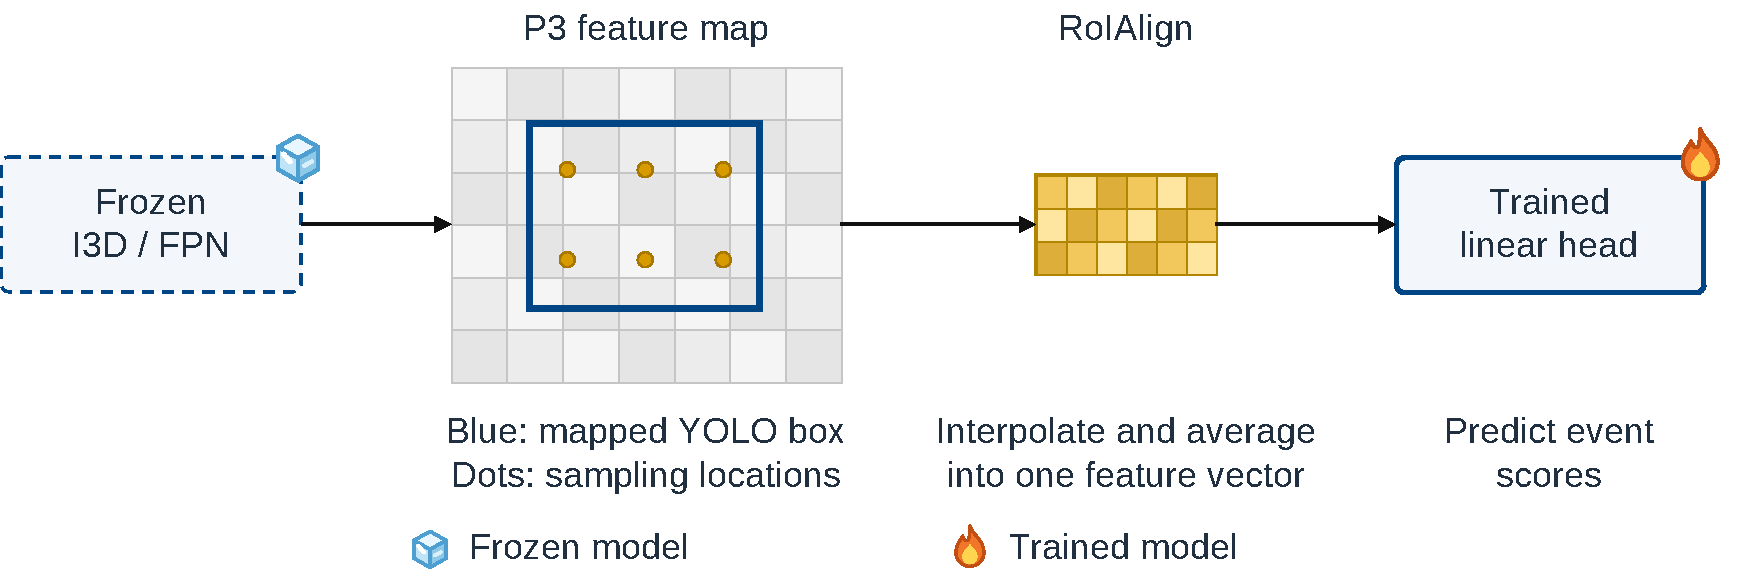
\includegraphics[width=\textwidth,height=0.60\textheight,keepaspectratio]{Fig/roi-align.pdf}
\caption[RoIAlign extraction at a proposed box.]{RoIAlign extraction at a proposed box.}
\label{fig:roi-align}
\end{figure}

A linear layer maps each vector to 184 logits. Training uses ground-truth boxes with multi-hot targets, random background boxes, and an additional set of YOLO background candidates. Background targets are zero across the output vector. The reported configuration uses focal classification loss with class-dependent alpha weights and focusing parameter \(\gamma = 2\) \cite{focal-loss}. The optional logical-penalty coefficient is zero in this configuration.

During evaluation, the head’s action, location, and composition sigmoids are multiplied by YOLO confidence. For a candidate with confidence q and raw class score p, the emitted score is qp. This gate affects detection ranking; it should not be interpreted as proof of calibrated probability. YOLO remains responsible for the emitted agentness and hard agent class. The Stage 1-to-2 transition changes feature access, the trained classifier, and confidence gating; it is not a feature-access-only ablation.

\section{Stacked Composition Learning}

Stage 3 keeps the Stage 2 feature extractor and full-data head fixed at evaluation. It concatenates 49 ungated primitive scores with the 256-dimensional pooled feature, producing a 305-dimensional input. A two-layer MLP, Linear(305,512) \(\rightarrow\) ReLU \(\rightarrow\) Linear(512,135), predicts 49 duplex and 86 triplet logits. Its sigmoid outputs replace only the composition columns.

The MLP is trained using video-grouped, two-fold out-of-fold predictions. These internal training folds do not replace the held-out validation split; the procedure is detailed below.

At evaluation, the full-training-data head supplies primitive predictions. The MLP receives raw, ungated sigmoids and the pooled feature. Its composition scores are gated by YOLO confidence only at emission. This ordering matches the representation used to train the MLP. Action and location pass through from Stage 2, and YOLO boxes and agent outputs remain unchanged.

Figure~\ref{fig:out-of-fold} details the training-only procedure, following the principle of stacked generalization \cite{stacking}. Training videos are assigned to two folds. A temporary linear head trained on fold A supplies predictions for fold B, and the head trained on fold B supplies predictions for fold A. The composition MLP therefore learns from predictions on videos excluded from the corresponding temporary head\textquotesingle{}s training set. Grouping by video prevents adjacent frames from being split between the two folds. The held-out designation applies to these temporary heads; the visual backbone is a shared frozen representation. The temporary heads are discarded after generating the MLP training inputs.

\begin{figure}[htbp]
\centering
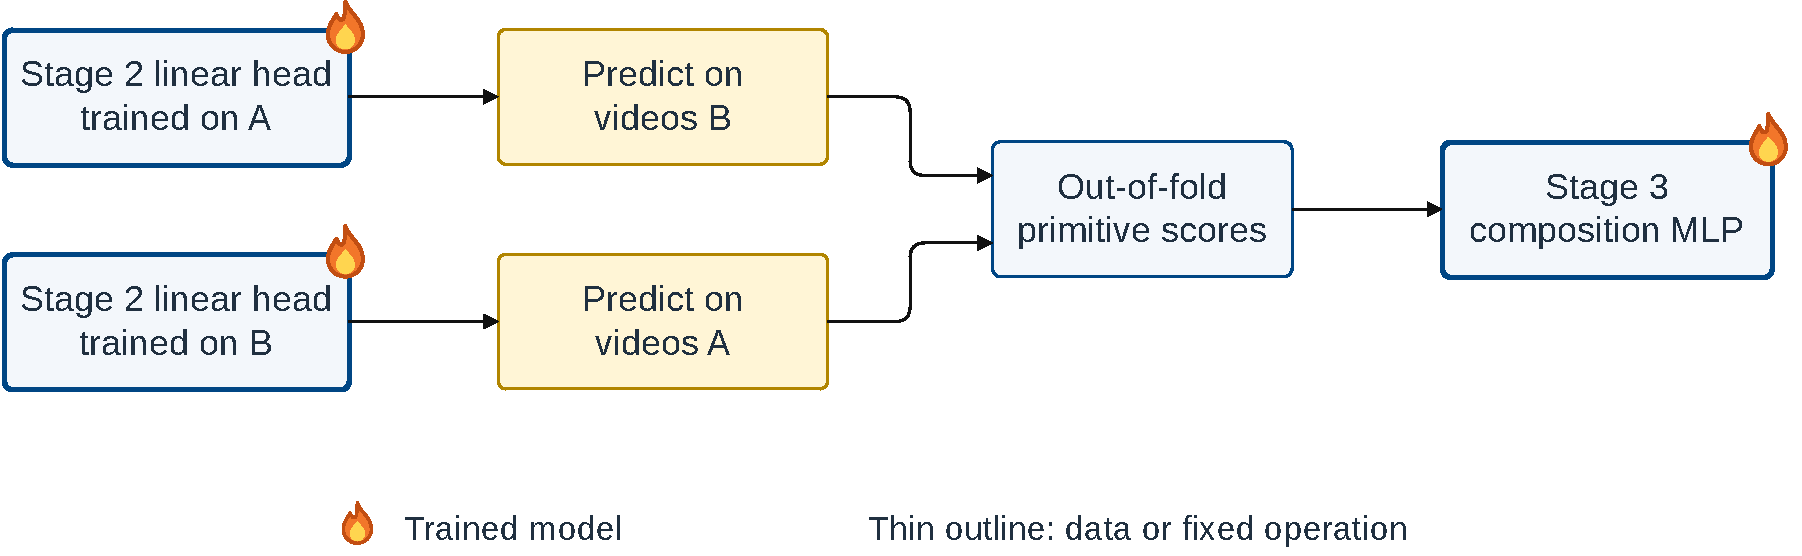
\includegraphics[width=\textwidth,height=0.60\textheight,keepaspectratio]{Fig/out-of-fold.pdf}
\caption[Video-grouped out-of-fold inputs for composition learning.]{Video-grouped out-of-fold inputs for composition learning, adapted from the stacking principle \cite{stacking}. A and B are folds of the training split.}
\label{fig:out-of-fold}
\end{figure}

Figure~\ref{fig:composition-detail} distinguishes learning a composition from replacing the entire prediction vector. The MLP receives 49 ungated scores---agentness plus agent, action, and location---together with 256 regional features. Its 135 outputs replace only the 49 duplex and 86 triplet entries. The feature input supplies visual evidence when primitive scores alone are ambiguous; retaining the remaining outputs makes the Stage 2-to-3 comparison specific to composition learning.

\begin{figure}[htbp]
\centering
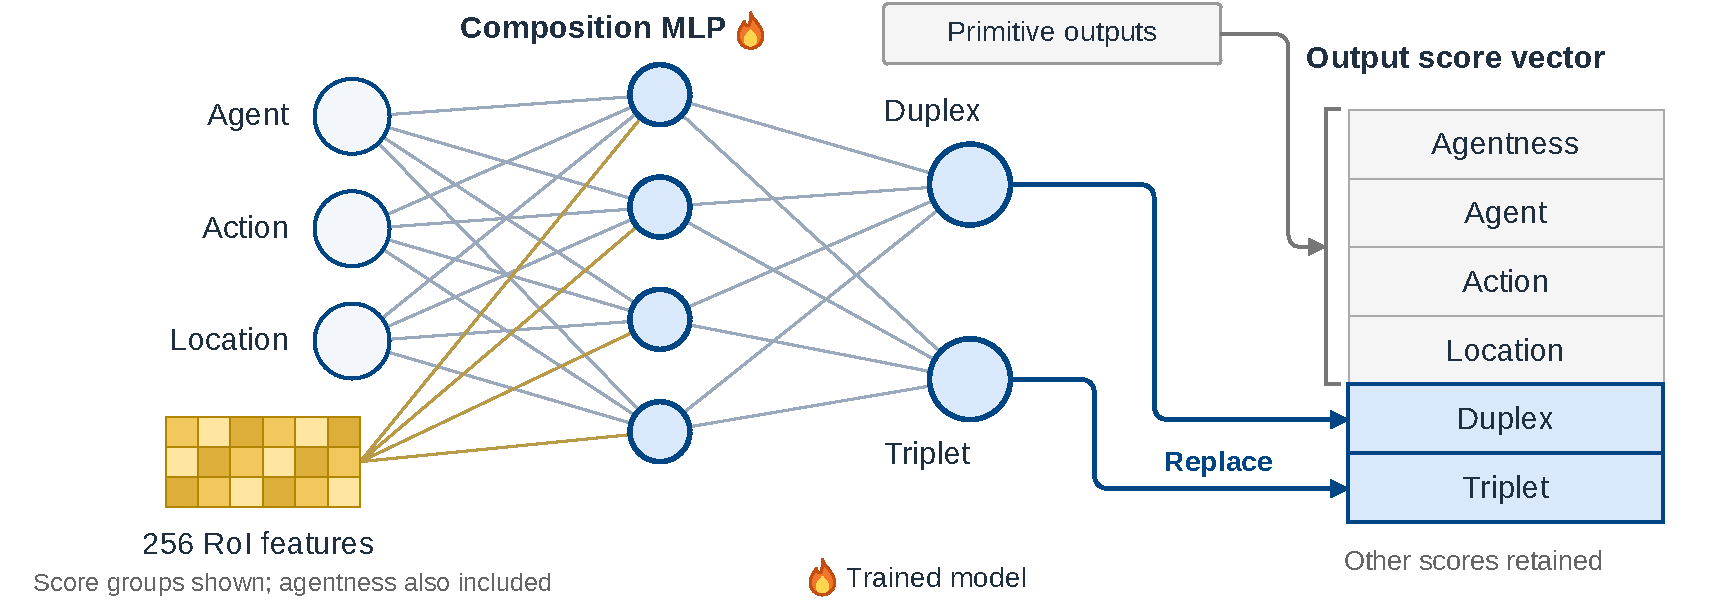
\includegraphics[width=\textwidth,height=0.60\textheight,keepaspectratio]{Fig/composition-detail.pdf}
\caption[Composition learning and selective output replacement.]{Composition learning and selective output replacement.}
\label{fig:composition-detail}
\end{figure}

The output vocabulary includes only the valid benchmark compositions. A nonexistent tuple has no dedicated output column. This vocabulary restriction does not guarantee agreement between independently scored primitives and compositions; cross-head consistency is a separate property.

Figure~\ref{fig:6} summarizes the completed Stage 3 architecture. Its composition module builds on the Stage 2 representation while preserving boxes and primitive outputs, providing the reference point for the results in Chapter 4.

\begin{figure}[htbp]
\centering
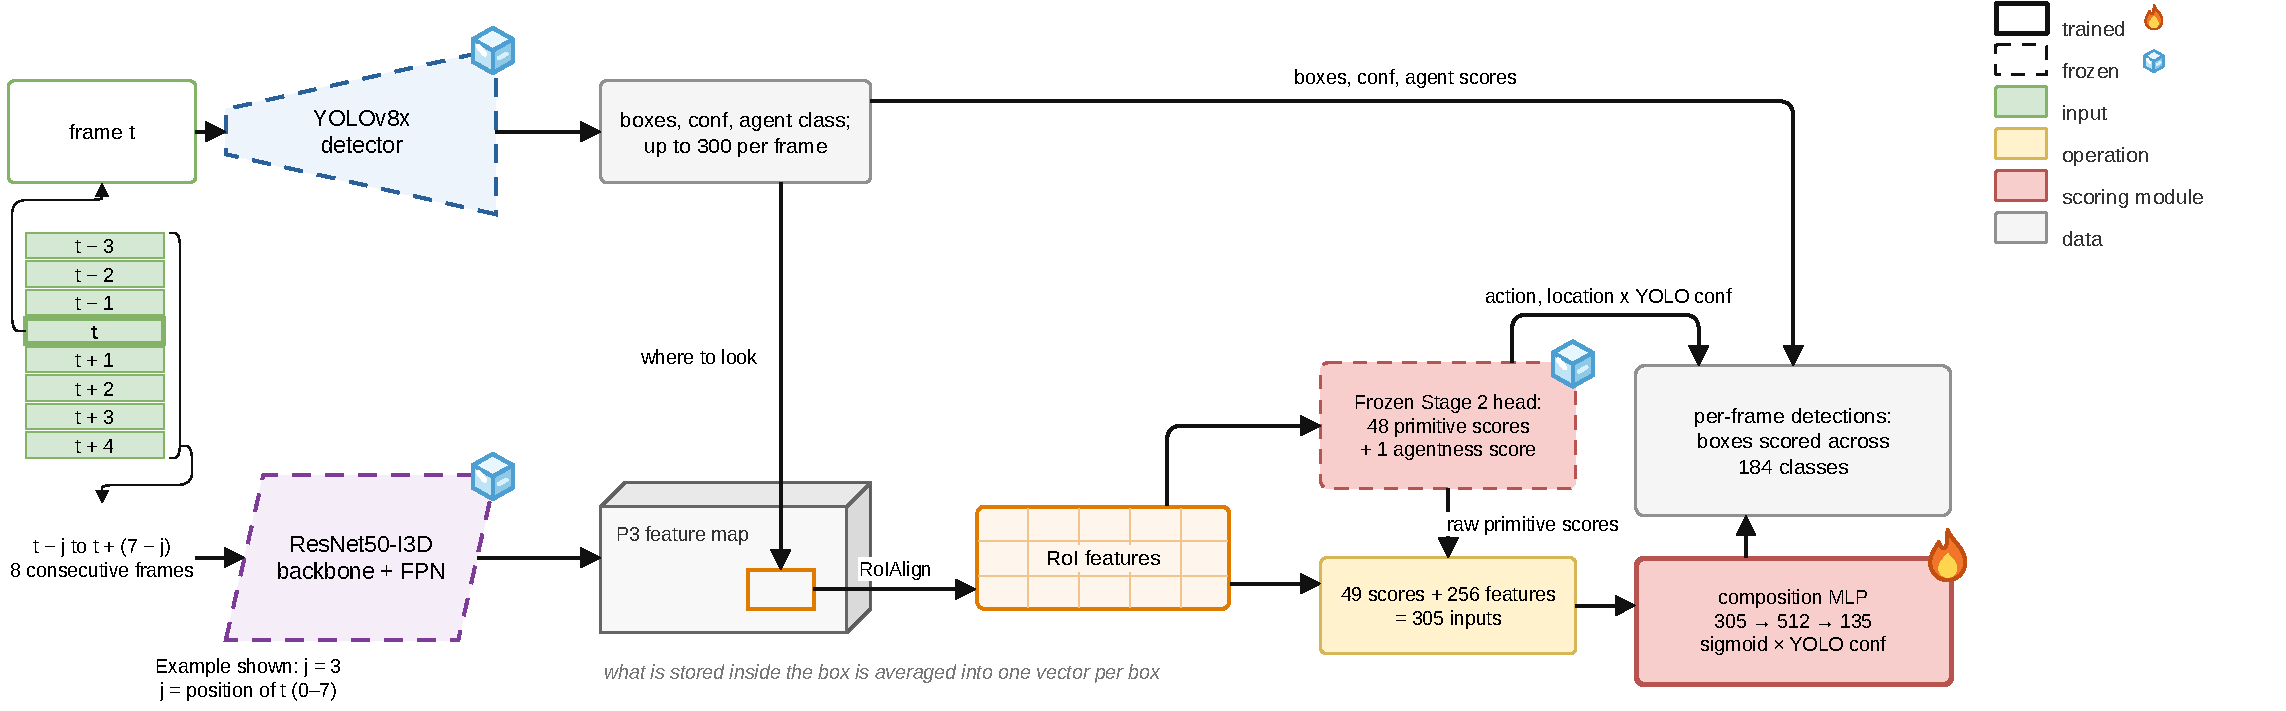
\includegraphics[width=\textwidth,height=0.68\textheight,keepaspectratio]{Fig/stage3-composition.pdf}
\caption{Completed Stage 3 learned-composition architecture.}
\label{fig:6}
\end{figure}

\section{Reproducibility and Label Integrity}

The source implementation fixes the 184-column ordering across frozen feature outputs, prediction heads, and evaluation. YOLO boxes are normalized coordinates; baseline boxes stored in an 840 \(\times\) 600 convention are converted before overlap calculations. These conventions are necessary for meaningful box matching and score assembly.

Valid compositions are derived from benchmark label names and the verified constraints file. The legacy duplex\_childs and triplet\_childs arrays are not used as authoritative mappings. Experiment records will retain the exact class order, candidate and feature identities, seeds, and evaluation manifests.

\chapter{Preliminary Results and Discussion}

Table~\ref{tab:3} reports the completed Stages 0--3 under the shared-frame protocol. The values are validation f-mAP percentages at IoU 0.5 on the same 36,717 frames. Stage 0 uses its own baseline candidates; Stages 1--3 reuse the fixed YOLO candidates. The results are project measurements.

\begin{table}[htbp]
\centering
\caption{Completed-stage validation f-mAP (\%).}
\label{tab:3}
\begin{singlespace}
\begin{tabular}{@{}lrrrr@{}}
\toprule
\textbf{Output} & \textbf{Stage 0} & \textbf{Stage 1} & \textbf{Stage 2} & \textbf{Stage 3} \\
\midrule
Agentness & 35.36 & 65.36 & 65.36 & 65.36 \\
Agent & 16.67 & 35.25 & 35.25 & 35.25 \\
Action & 13.23 & 12.86 & 15.92 & 15.92 \\
Location & 12.77 & 13.36 & 19.60 & 19.60 \\
Duplex & 11.32 & 10.04 & 11.13 & 15.52 \\
Triplet & 7.54 & 6.81 & 6.65 & 9.73 \\
\bottomrule
\end{tabular}
\end{singlespace}
\end{table}

The detector substitution raises agent f-mAP from 16.67\% to 35.25\%. However, improved agent detection does not automatically improve compositions. Stage 1 reaches 6.81\% triplet f-mAP, below the Stage 0 value of 7.54\%, while retaining the baseline-detection matching dependency. This comparison does not isolate that dependency’s contribution from changes in candidates and score construction.

Stage 2 removes that matching dependency and improves action and location f-mAP to 15.92\% and 19.60\%. Its free composition columns reach 11.13\% duplex and 6.65\% triplet f-mAP. This separates two observations: the region features support improved primitive classification, but the independently learned composition scores still leave a substantial gap.

\section{Effect of Learned Composition}

Stage 3 increases duplex f-mAP from 11.13\% to 15.52\% and triplet f-mAP from 6.65\% to 9.73\%, while boxes, agentness, agent, action, and location outputs remain unchanged. The changes are 4.39 and 3.08 percentage points for duplex and triplet, respectively. Relative to Stage 0, Stage 3 is higher on all six output groups in this comparison.

The auxiliary composition comparison provides additional context. An MLP using primitive scores alone reaches 13.37\% duplex and 8.93\% triplet f-mAP; adding the 256-dimensional visual feature raises those values to 15.52\% and 9.73\%. Fixed minimum composition gives 10.36\% and 5.52\%, while corrected single-gate product composition gives 10.58\% and 6.05\%. These measurements support learning composition from both primitive evidence and visual features in this setting. They do not establish a universal advantage over every possible structured model.

\section{Rare-Composition Performance and Limitations}

Table~\ref{tab:4} separates the overall triplet result from the training-count-defined tail. The \(z < 0\) group contains 47 classes and the \(z < -0.5\) group contains 28 of those same classes. These memberships remain fixed across stages.

\begin{table}[htbp]
\centering
\caption{Overall and tail triplet AP (\%).}
\label{tab:4}
\begin{singlespace}
\begin{tabular}{@{}lrrrr@{}}
\toprule
\textbf{Triplet group} & \textbf{Stage 0} & \textbf{Stage 1} & \textbf{Stage 2} & \textbf{Stage 3} \\
\midrule
All 86 & 7.54 & 6.81 & 6.65 & 9.73 \\
\(z < 0\) (47) & 4.14 & 3.43 & 2.60 & 4.53 \\
\(z < -0.5\) (28) & 2.88 & 2.19 & 1.47 & 3.31 \\
\bottomrule
\end{tabular}
\end{singlespace}
\end{table}

Stage 3 recovers the tail losses seen in Stages 1 and 2 and exceeds the Stage 0 primary-tail result by 0.39 percentage points.

The controlled Stage 2-to-3 comparison is particularly informative for the rare-event question: primary-tail AP rises from 2.60\% to 4.53\%, a gain of 1.93 percentage points, while deeper-tail AP rises from 1.47\% to 3.31\%, a gain of 1.84 points. Candidate boxes and primitive outputs are fixed in this comparison, so these gains accompany the learned-composition replacement rather than a new detector. Nevertheless, primary-tail AP remains 4.53\%, compared with 9.73\% over all triplets. The deeper-tail value is 3.31\%. This is the central empirical motivation for Stage 4: gains in overall composition recognition leave rare-event performance low.

The difference between overall and tail means is descriptive. It is not a significance test, nor is it direct evidence that language will solve the remaining problem. The proposed study asks whether semantic structure helps under controls that separate it from representation and classifier changes.

The completed sequence demonstrates that localization, feature access, and composition learning have different effects. Stage 1 changes localization and agent outputs but preserves a detection-matching bottleneck. Stage 2 obtains features for every candidate. Stage 3 changes composition predictions while preserving the earlier outputs. This last transition is the strongest controlled comparison for the learned-composition claim.

These are results on a shared validation population used during development. They do not constitute independent test-set confirmation, a tube-level leaderboard submission, or evidence of real-world driving safety. The completed table also does not establish repeated-seed significance. Accordingly, the proposal treats it as preliminary evidence supporting a focused investigation rather than as a final generalization claim.

\chapter{Conclusion and Future Work}

This thesis investigated long-tail compositional road-event detection using a decoupled detector and event classifier. The completed study extends from a replicated joint detector through direct regional classification, learned composition, semantic crop classification, and contextual expert blending. The results show that improved agent localization alone does not resolve event recognition: early score transfer improves agent detection while reducing triplet mAP. Direct feature access and learned composition provide a stronger basis for subsequent semantic and contextual models.

\section{Principal Findings}

Learned composition improves the controlled Stage 2-to-3 comparison from 6.65\% to 9.73\% triplet mAP while keeping candidate boxes and primitive outputs fixed. Semantic crop classification reaches 5.77\% tail mAP, but its 9.07\% overall triplet result remains below Stage 3. Adding phrase-composition evidence to the crop composition MLP changes triplet mAP only from 11.23\% to 11.28\%, with a deeper-tail regression. These findings motivate evaluating overall, common, and rare-class behavior separately.

The contextual family combines crop features, actor-region evidence, the wider scene, box geometry, and phrase representations. Original-encoder language controls favor the real phrase bank on tail means, while their small sample and geometry differences limit a purely semantic interpretation. Classification-only contextual heads already use language; the additional contrastive objective makes small, mixed changes. Its value in the final model includes complementarity with a separately trained classification expert.

The final Contextual Semantic Expert Blend achieves \(15.75\pm0.27\)\% triplet mAP and \(9.00\pm0.64\)\% tail mAP across three seeds, where the uncertainty term is sample standard deviation. Relative to the original-encoder DCB blend, the mean increases are 2.32 percentage points overall and 2.77 points on the tail. Approximately 65\% of the overall improvement comes arithmetically from the 47 tail classes, and common-class performance also improves. This result supports the final system under the fixed validation protocol; it does not isolate encoder size, language, or loss as the sole cause.

\section{Limitations}

The evaluation population is a shared subset of ROAD-Waymo validation used during development. Checkpoint selection and blend fitting use held-out training videos, but subsequent research decisions were informed by validation results. Three repeated seeds measure optimization sensitivity on this fixed population and do not establish environmental generalization. Published comparisons differ in candidates, filtering, training, and repetition counts, so higher reported mAP does not constitute a matched state-of-the-art test.

The scaling comparison changes both pretrained towers, the text projection, and cache precision. Language-bank controls reported here concern the original-encoder focal scene-attention head. They cannot establish the same effect in the scaled DCB blend. The fixed class vocabulary does not test unseen combinations, and valid composition columns do not guarantee agreement with independently scored primitives. The study also does not establish end-to-end real-time performance or driving safety.

\section{Future Work}

Matched language-bank controls in the scaled CSEB, followed by separate visual- and text-checkpoint comparisons, would narrow the attribution of the final gains. These comparisons should hold cache precision and head interfaces fixed. Additional seeds and an independent evaluation population would strengthen reproducibility and generalization claims.

Per-class analysis should identify persistent rare-composition errors and distinguish recognition failures from missing or inaccurate boxes. Causal temporal windows, cross-domain evaluation, and full-pipeline latency measurements are needed before online use. Structured output constraints could test consistency separately from AP.

\clearpage
\printbibliography[heading=bibintoc,title={References}]
\clearpage
% No appendix content is present; the official template permits omission.
\end{document}
